\documentclass[a4paper,14pt]{extarticle}
\usepackage{graphicx}
\usepackage{times}
\usepackage{geometry}
\usepackage{amssymb}
\usepackage{amsmath}
\usepackage{multirow}
\usepackage{tabularx}
\usepackage{longtable}
\usepackage{fontspec}
\usepackage{natbib}
\usepackage{ragged2e} % not needed for now
\usepackage{hyperref} % make table of contents clickable
\usepackage[nottoc]{tocbibind} % add bibliography to ToC

% Set languages and fonts
\usepackage{polyglossia}
\setdefaultlanguage{ukrainian}
\setotherlanguage{english}
\setotherlanguage{russian}
\newfontfamily\cyrillicfont{Times New Roman}[Script=Cyrillic]
\newfontfamily\cyrillicfontsf{Times New Roman}[Script=Cyrillic]
\newfontfamily{\cyrillicfonttt}{Times New Roman}

\addto\captionsukrainian{
  \renewcommand{\bibname}
    {Список літературних джерел}
}

\geometry{
	a4paper,
	left=30mm,
	top=20mm,
	right=20mm,
	bottom=20mm,
}

\hypersetup{
	colorlinks,
	allcolors=black,
}

\renewcommand{\baselinestretch}{1.5}

\begin{document}

\title{Метод автоматизованої класифікації текстових даних на основі гібридних моделей}
\author{Misha Behersky}

\tableofcontents
\newpage

\begin{center}
	\textbf{\uppercase{Анотація}}
\end{center}

Дана магістерська дисертація присвячена розробці методу автоматизованої класифікації текстових даних на основі гібридних моделей. 

Даний проект складається з двох основних частин: ресурсу для збору початкових даних та компоненту, що здійснює тренування та запуск моделей на отриманих даних. Частина для агрегації вхідних даних являє собою веб-додаток, що використовується для проходження опитування і формуванні результуючої таблиці на основі заповних форм. В якості проміжного етапу здійснюється підготовка та попередня обробка даних для подальшого використання. Підсистема класифікації в свою чергу поділена на два підмодуля: безпосередня імплементація розробленого методу класифікації та використання побудованої моделі для прогнозування зміни досліджуваної величини.

В рамках магістерської дисертації проведено аналіз існуючих систем для збору даних та розробка власної системи на основі адаптації готових рішень під вимоги досліджуваної області. Було здійснено дослідження існуючих алгоритмів для класифікації текстових даних та алгоритмів і бібліотек, що використувуються для побудових моделей прогнозування. Проведено оцінку предметної області, сформовано функціональні та нефункціональні вимоги до програмного забезпечення, а також проаналізовано перспективи виходу на ринок та запуску даного проекту в комерційних цілях.

У даній магістерській дисертації розроблено: архітектуру веб-ресурсу, інтерфейс для збору початкових даних, компнонент для обробки та трансформації даних, алгоритм для побудови прогностичної моделі та утиліту командного рядка для прикладного запуску моделі в якості інструменту прогнозування зміни цільової величини вхідних даних. Виконаний порівняльний аналіз з уже існуючими рішеннями та перевірка коректності роботи на основі порівняння відхилення результуючих показників з еталонними. Дана система готова розгортання, використання та інтеграції з іншими рішеннями, а також до впровадження в якості самостійного проекту на ринок, націленого на комерціалізацію продукту.


\newpage
\begin{center}
	\textbf{\uppercase{Abstract}}
\end{center}

This Master's dissertation is about creating a method for automatic text data classification based on blender models.

The project consists of two main parts: data collection module and a compoment responsible for training and launching a model on the input data. Subcomponent for input data aggregation is a web-application that is used by target users to take a survey and then to form a resulting table based on an information filled. As a part of main pipeline data transformation and preprocessing takes place. Classification system by its own consists of two connected modules: implementation of a classification method and application for prediction using the model built.

In the scope of dissertation analysis of current system for data mining was made. Also new project based on requirements from domain field using solutions from existing alternatives was created. Research on existing algorithms of text data classification and comparison of libraries was conducted. The research in the domain field was performed, functional and non-functional requirements for the software were generated. Possibilities for commercial launching of the project were considered and corresponding breakdown took place.

Within the Master's dissertation following components were created: architecture of a web-resource, user interface for collecting initial data, component for data transformation and preprocessing, algorithm for predictive model creation, command line utility for launching a model built on the dataset in order to predict target value. Developed solution was compared to competitors and final measurements about system's correctness was made based on reference data. System created is ready for deployment, direct usage and integration with existing solutions as well as moving forward to the market targeting commercialization of a product.

\newpage
\begin{center}
	\textbf{\uppercase{Аннотация}}
\end{center}

Данная магистерская диссертация посвящена разработке метода автоматизированной классификации текстовых данных на базе гибридных моделей.

Проект состоит из двух основных частей: ресурсы для сбора начальных данных и компонента, отвечающего за тренировку и запуск моделей на существующих данных. Часть агрегации данных представляет собой веб-приложение, которое испльзуется для прохождения опроса и формирования финальной таблицы на основании заполненых форм. В качестве промежуточного этапа производится подготовка и дообработка данных для дальнейшего использования. Система классификации в свою очередь разделена на два модуля: непосредственная имплементация разработанного метода классификации и использование построенной модели для прогнозирования изменений исследуемого значения.

В рамках диссертации проведен анализ существующих систем для сбора данных, а также разработана собственная система на основании адаптации готовых решений к требованиям предметной области. Осуществлено исследование алгоритмов классификации текстовых данных, а также алгоритмов и библиотек, которые используются для построения прогностических моделей. Проведено оценку предметной области, сформировано функциональные и нефункциональные требования к программному продукту, а также проанализировано перспективы выхода на рынок и запуска проекта в коммерческих целях.

В магистерской диссертации разработано: архитектуру веб-ресурса, интерфейс для сбора начальных данных, компонент для обработки и трансформации данных, алгоритм построения прогностической модели и утилиту командной строки для запуска модели в качестве инструмента прогнозирования изменений целевого значения входящих данных. Был осуществлен анализ с уже существующими решениями и проверка корректности работы на основании сравнения отклонения результатов с еталонными значениями. Система полностью готова к разворачиванию, использованию и интеграции с другими продуктами, а также к внедрению в качестве самостоятельного решения с целью коммерциализации проекта.

\section{Вступ}
Зі стрімким ростом об'єму інформації онлайн, класифікація тексту стала однією з ключових
технік для обробки та впорядкування даних. Галузі застосування є досить широкими:
починаючи від класифікації новин і закінчуючи персоналізованим пошуком відповідно до
потреб користувача. Оскільки побудова власного класифікатору є досить складним та
часозатратним процесом, доцільно розглянути приклади уже існуючих класифікаторів.
На сьогоднішній день існує величезна кількість алгоритмів, що використовуються для побудови прогностичних моделей. Прогностичні моделі – це математичні методи, що використовують статистику для передбачення майбутніх значень досліджуваної величини. Побудова таких моделей частіше за все здійснюється з метою передбачення поведінки величини у майбутньому, але загалом можуть бути використані для будь-якого типу події, незалежно від часу, коли вона відбулася.

\subsection{Прогностичне моделювання}
Прогностичне моделювання – використання статистичних методів для передбачення деякого цільового значення. Зазвичай, мається на увазі передбачення деякої величини в майбутньому, хоча узагальнено це не грає жодної ролі і може бути застосовано до будь-якого типу невідомої події, незалежно від того, коли вона відбулася.

В багатьох випадках задача зводиться до вибору найкращої моделі, що намагається здогадатися результат на основі набору вхідних даних, наприклад визначення того, чи є деякий лист електронної пошти спамом. Моделі можуть використовувати один чи декілька класифікаторів, щоб визначати приналежність даних до деякої множини. Сам термін прогностичної моделі широко перетинається з поняттями машинного навчання в наукових статтях та в контексті розробки програмного забезпечення. В промисловому середовищі даний термін швидше відноситься до поняття прогностичного аналізу.

Будь-яка регресійна модель може бути використана для прогностичних моделей. Загалом можна говорити про два класи прогностичних моделей: параметризовані та непараметризовані. Існує також суміжний третій клас, що поєднує властивості обох попередніх. Основна відмінність полягає в тому, що параметричні моделі роблять "визначені припущення, спираючись на один чи декілька параметрів, що характеризують закладений розподіл", в той час як непараметризовані не роблять жодних припущень на основі розподілу.

\subsubsection{Представлення та використання результатів прогностичних моделей}
Прогностичні моделі можуть бути використані безпосередньо, щоб отримати відповідь (результат) на основі вхідних характеристик (даних) або як компонент при здійсненні вибору на основі деяких правил.

В залежності від методології, що використовується для прогнозування, часто можна вивести деяку формулу-узагальнення (апроксимацію), що може бути використана в будь-якому додатку для роботи з таблицями. Це дає змогу працювати зі складними алгоритмами людям з досвідом роботи лише у офісних документах.

Номограми – графічні представлення прогностичних моделей. Перевагою такого представлення є можливість використання моделі без необхідної участі комп'ютера. Наприклад, деяка крива може бути використана на координатній площині для знаходження певної потрібної точки.

Дискретні оцінки – таблиця-представлення і найпростіший спосіб використання моделі. В рядках задається необхідне вхідне значення та вихідний параметр відповідно відображається в іншій колонці. Це може бути звичайна таблиця або деякий граф.

Окремим класом представлення є комп'ютерні додатки та веб-орієнтовані додатки, що дають аналогічне представлення у вигляді комп'ютерної програми з тюнінгом параметрів в режимі реального часу.

\subsubsection{Моделі росту}
Моделювання росту – це техніка, що показує зміну ймовірності в результаті певних дій. Наприклад, визначення того, чи клієнт залишиться покупцем певної компанії після випуску нового продукту. Модель дозволить вибрати оптимальну стратегію реклами серед покупців і економії грошей на існуючих клієнтах, що за даними прогностичної моделі залишаться покупцями незалежно від дій компанії.

Моделі, що будуються для визначення ймовірності прийняття клієнтом тих чи інших рішень. Використовуються для утримання клієнтів, маркетингу та продажів.

Модель може бути використана для оцінки ризиків виникнення інцидентів. Наприклад, дані про характеристики автомобіля та водійського стажу можуть слугувати показником ймовірності потрапляння в аварію.

Показники з медичних записів та історії хвороб пацієнтів можуть описувати моделі для визначення ризику виникнення захворювання чи необхідності повторного лікування.

Визначення ключових змінних, що впливають на ціну акцій, стоків, фьючерсів та курсу валют може бути використане для створення моделі, що побудує стратегію торгів та дасть змогу побудувати шаблони розвитку ринку. Щоправда, наразі невідомо жодної моделі, що на основі попередніх історичних даних могли б дати необхідні показники для успішної торгівлі на ринку.

Історичних даних не завжди достатньо для передбачення майбутніх даних. Використовуючи такі припущення ми вважаємо, що система має константні величини, від яких залежить система, що завжди хибни за умови участі людського фактору в будь-якій системі.

Не важливо, скільки факторів було враховано при зборі даних, завжди існує ймовірність, що нова, раніше не врахована змінна, викличе значний вплив на систему в майбутньому, що буде критично для попередньо розрахованих значень моделі.

Самопідтвердження алгоритму – якщо деякий алгоритм буде прийнято стандартом для вимірювань, особи, що мають інформацію про властивості алгоритму можуть використати його в особистих цілях та в цілях маніпуляції змінними, що не враховані в даному алгоритмі.

Лінійна регресія - статистичний метод, що дозволяє узагальнити та вивчати зв'язки між двома неперервними величинами. Одна з досліджуваних величин є незалежною, а інша - вихідна величина, залежна змінна, значення якої ми зазвичай хочемо отримати. Це найпростіша форма моделі, яка враховує лише одну характеристичну величину. Для лінійної регресії важливо знайти функціональний зв'язок між цими величинами (рис. \ref{fig:linear_regression}), наприклад зв'язок між температурою за шкалою Фаренгейта та Цельсія виражається такою формулою: $Fahr = 9/5Cels + 32$.

\begin{figure}[h!]
  \centering
  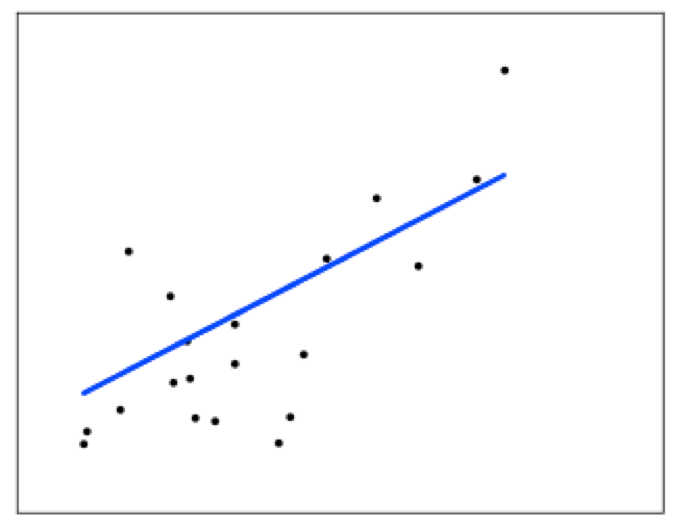
\includegraphics[width=0.9\linewidth]{figures/linear_regression.png}
  \caption{Візуалізація лінійної регресії}
  \label{fig:linear_regression}
\end{figure}

Для різного роду бізнес задач, підприємств та процесів загалом необхідність моделювання та передбачення деяких цільових значень стає ключовим фактором, на якому будується комплексна система. Ефективність даної системи прямопропорційно зв'язана з точністю даних, що будуть спрогнозовані, а тому використання найкращих алгоритмів є досить актуальною задачею. За рахунок росту об'єму даних, які вимагають обробки та прогнозування виникає і інший фактор, що насамперед ставить вимогу до швидкодії використовуваного алгоритму. Саме тому необхідність створення універсальної прогностичної моделі з гарними показниками передбачення та швидкодії стоїть на одному з перших місць у списку як для науковців, так і для користувачів, що будуть застосовувати дану модель у прикладних цілях.

\section{Теоретичні основи е-е}
На відміну від штучно створених мов, наприклад мов програмування чи математичних нотацій,
мови, які ми використовуємо для спілкування, розвивалися з покоління в покоління, постійно
видозмінюючись, а тому досить складно відслідкувати і встановити набір чітких конкретно
визначених правил. Розробка алгоритмів, що дозволяють "розуміти" людські висловлювання
дає змогу покращити велику кількість аспектів взаємодії людини та комп'ютера: передбачення
вводу, розпізнавання тексту, пошук інформації в неструктурованому тексті, переклад з однієї
мови на іншу, аналіз емоційного забарвлення тексту та багато іншого. Створюючи інтерфейси,
що дозволяють людині більш ефективно використовувати комп'ютер, ми прискорюємо
розвиток багатомовного інформаційного суспільства.

\subsection{Методи класифікації даних}

\subsubsection{Проблема класифікації даних}
Задача класифікації – формалізована задача, яка містить множину об’єктів (ситуацій), поділених певним чином на класи. Задана кінцева множина об'єктів для яких відомо, до яких класів вони відносяться. Ця множина називається вибіркою. До якого класу належать інші об'єкти невідомо. Необхідно побудувати такий алгоритм, який буде здатний класифікувати довільний об'єкт з вихідної множини.
Класифікувати об'єкт – означає вказати номер (чи назву) класу, до якого відноситься даний об'єкт.
Класифікація об'єкта – номер або найменування класу, що видається алгоритмом класифікації в результаті його застосування до даного конкретного об'єкту.
В математичній статистиці задачі класифікації називаються також задачами дискретного аналізу. В машинному навчанні завдання класифікації вирішується, як правило, за допомогою методів штучної нейронної мережі при постановці експерименту у вигляді навчання з учителем (supervised machine learning).
Існують також інші способи постановки експерименту – навчання без вчителя (unsupervised learning), але вони використовуються для вирішення іншого завдання – кластеризації або таксономії. У цих завданнях поділ об'єктів навчальної вибірки на класи не задається, і потрібно класифікувати об'єкти тільки на основі їх подібності. У деяких прикладних областях, і навіть у самій математичній статистиці, через близькість завдань часто не відрізняють завдання кластеризації від завдання класифікації.

Деякі алгоритми для вирішення задач класифікації комбінують навчання з учителем і навчання без вчителя, наприклад, одна з версій нейронних мереж Кохонена – мережі векторного квантування, яких навчають способом навчання з учителем.

Прогностичне моделювання – використання статистичних методів для передбачення деякого цільового значення. Зазвичай, мається на увазі передбачення деякої величини в майбутньому, хоча узагальнено це не грає жодної ролі і може бути застосовано до будь-якого типу невідомої події, незалежно від того, коли вона відбулася.
В багатьох випадках задача зводиться до вибору найкращої моделі, що намагається здогадатися результат на основі набору вхідних даних, наприклад визначення того, чи є деякий лист електронної пошти спамом. Моделі можуть використовувати один чи декілька класифікаторів, щоб визначати приналежність даних до деякої множини. Сам термін прогностичної моделі широко перетинається з поняттями машинного навчання в наукових статтях та в контексті розробки програмного забезпечення. В промисловому середовищі даний термін швидше відноситься до поняття прогностичного аналізу.

\subsubsection{Існуючі методи класифікації даних}
В залежності від вхідних даних, для задач класифікації можна виділити такі категорії:

\begin{itemize}  
	\item Характеристичний опис – найпоширеніший випадок. Кожен об'єкт описується набором своїх характеристик, які називаються ознаками. Ознаки можуть бути числовими або нечисловими.
	\item Матриця відстаней між об'єктами. Кожен об'єкт описується відстанями до всіх інших об'єктів навчальної вибірки. З цим типом вхідних даних працюють деякі методи, зокрема, метод найближчих сусідів, метод потенційних функцій.
	\item Часовий ряд або сигнал є послідовність вимірів у часі. Кожен вимір може представлятися числом, вектором, а в загальному випадку – характеристичним описом досліджуваного об'єкта в цей момент часу.
	\item Зображення або відеоряд.
\end{itemize}

Зустрічаються і складніші випадки, коли вхідні дані представляються у вигляді графів, текстів, результатів запитів до бази даних, і т. д. Як правило, вони приводяться до першого або другого випадку шляхом попередньої обробки даних та вилучення характеристик. Щодо класифікації сигналів та зображень, то її також називають розпізнаванням образів.

В залежності від кількості класів, на які розбиваються вхідні дані, отримуємо такий поділ:
\begin{itemize}  
	\item Двокласова класифікація (бінарна класифікація). Найпростіший в технічному відношенні випадок, який служить основою для вирішення складніших завдань.
	\item Багатокласова класифікація. Коли число класів досягає багатьох тисяч (наприклад, при розпізнаванні ієрогліфів або злитого мовлення), завдання класифікації стає істотно важчим.
	\item Непересічні класи.
	\item Пересічні класи. Об'єкт може належати одночасно до декількох класів.
	\item Нечіткі класи. Потрібно визначати ступінь належності об'єкта кожному з класів, звичайно це дійсне число від 0 до 1.
\end{itemize}

Прикладом одного з методів, що використовуэться найчастіше, є наївний баєсівський метод (байєсівський класифікатор). Наївна байєсівська модель є ймовірнісним методом навчання. Імовірність того, що документ $d$ потрапить у клас $c$ записується як $P(c|d)$.

\subsubsection{Машинне навчання з учителем}
Машинне навчання - узагальнена назва методів штучної генерації знань з досвіду. Штучна система навчається на прикладах і після закінчення фази навчання може узагальнювати. Тобто система не просто вивчає наведені приклади, а розпізнає певні закономірності в даних для навчання.

Серед багатьох програмних продуктів машинне навчання використовують: системи автоматичного діагностування, розпізнавання шахрайства з кредитними картками, аналіз ринку цінних паперів, класифікація ланцюжків ДНК, розпізнавання мовлення та тексту, автономні системи.

Машинне навчання — розділ штучного інтелекту, має за основу побудову та дослідження систем, які можуть самостійно навчатись з даних. Наприклад, система машинного навчання може бути натренована на електронних повідомленнях для розрізняння спам і не спам-повідомлень. Після навчання вона може бути використана для класифікації нових повідомлень електронної пошти на спам та не-спам папки.

В основі машинного навчання розглядаються уявлення та узагальнення. Представлення даних і функцій оцінки цих даних є частиною всіх систем машинного навчання, наприклад, у наведеному вище прикладі повідомлення по електронній пошті, ми можемо уявити лист як набір англійських слів, просто відмовившись від порядку слів. Існує широкий спектр завдань машинного навчання та успішних застосувань. Оптичне розпізнавання символів, в яких друковані символи розпізнаються автоматично, ґрунтуючись на попередніх прикладах, є класичним прикладом техніки машинного навчання. У 1959 році Артур Самуїл визначив машинне навчання як “Поле дослідження, яке дає комп'ютерам можливість навчатися, не будучи явно запрограмованим” \cite{book:arthur_samuel}.

Практичне використання відбувається, переважно, за допомогою алгоритмів. Різноманітні алгоритми машинного навчання можна грубо поділити за такою схемою:
\begin{itemize}  
	\item Навчання з вчителем – алгоритм вивчає функцію на основі наданих пар вхідних та вихідних даних. При цьому, в процесі навчання, «вчитель» вказує вірні вихідні дані для кожного значення вхідних даних. Одним з розділів навчання з вчителем є машинна класифікація. Такі алгоритми застосовуються для розпізнавання текстів.
	\item Багатокласова класифікація. Коли число класів досягає багатьох тисяч (наприклад, при розпізнаванні ієрогліфів або злитого мовлення), завдання класифікації стає істотно важчим.
	\item Навчання без вчителя.
	\item Пересічні класи. Об'єкт може належати одночасно до декількох класів.
	\item Навчання з закріпленням (англ. reinforcement learning): алгоритм навчається за допомогою тактики нагороди та покарання для максимізації вигоди для агентів (систем до яких належить компонента, що навчається).
\end{itemize}

Узагальнення в цьому контексті є здатність алгоритму для виконання точно на нових, невідомих прикладах після тренування на навчальному наборі даних. Основна мета учня узагальнювати свій досвід.

Також існує поняття інтелектуального аналізу даних, що за своєю природою відрізняється від машинного навчання. Два терміни часто плутають, оскільки вони не рідко використовують ті ж методи і перекриття. Вони можуть бути умовно визначені наступним чином: машинне навчання фокусується на прогноз, заснований на відомих властивостях, витягнутих з навчальних даних. Інтелектуальний аналіз даних (який є кроком виявлення знань у базах даних) фокусується на відкриття (раніше) невідомих властивостей даних.

Ці дві області перекриваються у багатьох відношеннях: інтелектуальний аналіз даних використовує безліч методів машинного навчання, але часто з дещо іншою метою. З іншого боку, машинне навчання також використовує методи інтелектуального аналізу такі як "неконтрольоване навчання" або як попередній крок оброблення для покращення точності навчальної системи. Велика частина плутанини відбувається з основних припущень: в машинному навчанні, виконання, як правило, оцінюється по відношенню до здатності відтворювати відомі знання, в той час як в інтелектуальному аналізі даних ключовим завданням є виявлення раніше невідомого знання. Необізнаний (неконтрольований) метод, який обчислюється по відношенню до відомих знань, буде легко перевершений керованими методами. В той час в типових ІАД завданнях, керовані методи не можуть бути використані через відсутність попередньої підготовки даних.

Деякі системи машинного навчання намагаються усунути необхідність в людській інтуїції під час аналізування даних, а інші обирають спільний підхід між людиною і машиною. Людська інтуїція не може бути повністю виключена, так як конструктору системи необхідно вказати, як дані повинні бути представлені і які механізми будуть використовуватися для пошуку характеристик даних.

Навчання з підкріпленням — це галузь машинного навчання натхненна біхевіористською психологією, що займається питанням про те, які дії мають виконувати програмні агенти в певному середовищі задля максимізації деякого уявлення про сукупну винагороду. Через свою загальність, дана проблема вивчається, вивчається багатьма іншими дисциплінами, такими як теорія ігор, теорія управління, дослідження операцій, теорія інформації, оптимізація на основі моделювання, багатоагентні системи, колективний інтелект, статистика та генетичні алгоритми. Галузь, що займається навчанням з підкріпленням, також називається наближеним динамічним програмуванням. Попри те, що проблема навчання з підкріпленням, вивчалась теорією оптимального управління, більшість досліджень стосувались саме існування оптимальних рішень та їх характеристики, а не навчання чи наближених аспектів. В економіці та теорії ігор, навчання з підкріпленням може використовуватись для пояснення того, як при обмеженій раціональності може виникати рівновага.

Навчання з учителем (англ. supervised learning) є одним із способів машинного навчання, в ході якого випробувана система примусово навчається за допомогою наявної множини прикладів «стимул-реакція» з метою визначення «реакції» для «стимулів», які не належать наявній множині прикладів. 

Між входами та еталонними виходами (стимул-реакція) може існувати деяка залежність, але вона невідома. Відома лише кінцева сукупність прецедентів – пар «стимул-реакція», звана навчальною вибіркою. На основі цих даних потрібно відновити залежність (побудувати модель відносин стимул-реакція, придатних для прогнозування), тобто побудувати алгоритм, здатний для будь-якого об'єкта видати досить точну відповідь. Для вимірювання точності відповідей, так само як і в навчанні на прикладах, може вводитися функціонал якості.

Задача машинного навчання може бути представлена у вигляді експерименту. Даний експеримент являє собою окремий випадок кібернетичного експерименту зі зворотним зв'язком. Постановка даного експерименту припускає наявність експериментальної системи, методу навчання і методу випробування системи або вимірювання характеристик.

Експериментальна система у свою чергу складається з випробовуваної (використовуваної) системи, простору стимулів одержуваних із зовнішнього середовища та системи управління підкріпленням (регулятора внутрішніх параметрів). В якості системи управління підкріпленням може бути використано автоматичний пристрій, що регулюють (наприклад, термостат), або людину-оператора (вчитель), здатну реагувати на реакції випробовуваної системи і стимули зовнішнього середовища шляхом застосування особливих правил підкріплення, що змінюють стан пам'яті системи.

Розрізняють два варіанти: (1) коли реакція випробовуваної системи не змінює стан зовнішнього середовища, і (2) коли реакція системи змінює стимули зовнішнього середовища. На рис. \ref{fig:experiment_system} зображено загальний вигляд такої експериментальної системи.
\begin{figure}[h!]
  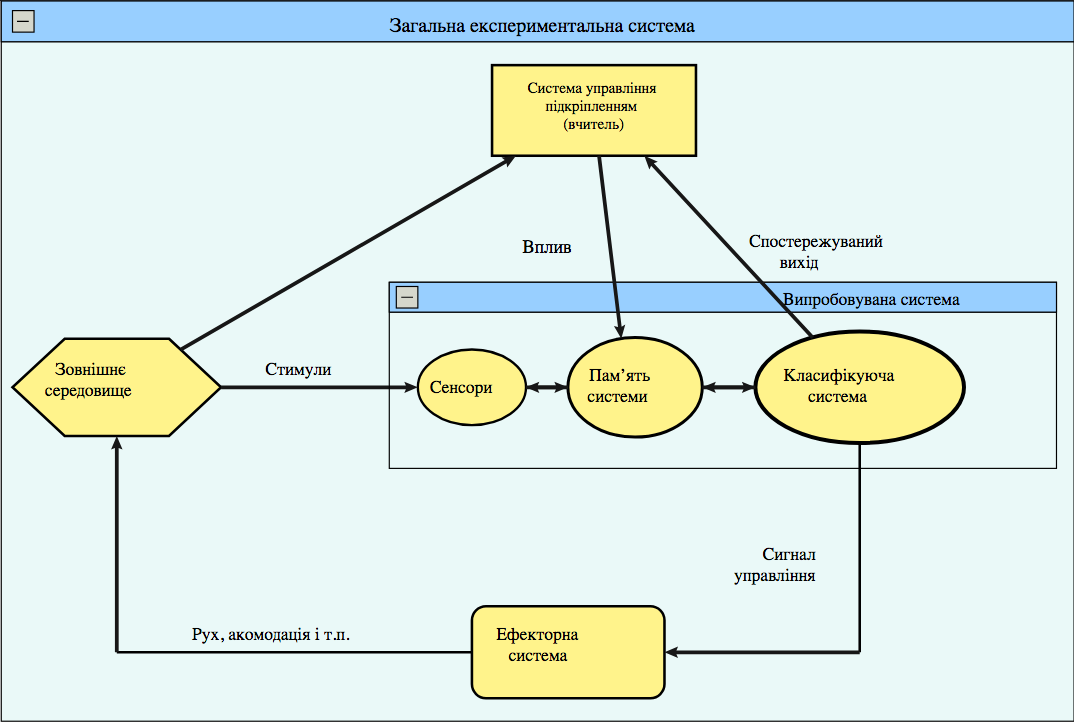
\includegraphics[width=\linewidth]{figures/fig_system.png}
  \caption{Експериментальна система для навчання з учителем}
  \label{fig:experiment_system}
\end{figure}

В залежності від результуючих даних, отриманих від системи, можна виділити такі категорії класифікуючих систем:
\begin{itemize}  
	\item Множина можливих відповідей нескінчення (відповіді є дійсними числами або векторами). В даному випадку говорять про задачі регресії та апроксимації.
	\item Множина відповідей звичайна – задача класифікації та розпізнавання образів.
	\item Відповіді характеризують майбутню поведінку процесу або явища. В цьому випадку мова йде про задачі прогнозування (прогностичне моделювання).
\end{itemize}

Існують також вироджені системи, які характеризуються дещо зміненою поведінкою підкріплення інформації ("вчителя"):
\begin{itemize}  
	\item Система підкріплення з керуванням по реакції (R — керована система) — характеризується тим, що інформаційний канал від зовнішнього середовища до системи підкріплення не функціонує. Дана система, незважаючи на наявність системи управління, відноситься до спонтанного навчання, оскільки випробовувана система навчається автономно, під дією лише своїх вихідних сигналів незалежно від їх "правильності". При такому методі навчання для управління зміною стану пам'яті не потрібно ніякої зовнішньої інформації.
	\item Система підкріплення з керуванням по стимулах (S — керована система) — характеризується тим, що інформаційний канал від випробовуваної системи до системи підкріплення не функціонує. Незважаючи на не функціонування каналу від виходів випробовуваної системи, відноситься до навчання з учителем, оскільки в цьому випадку система підкріплення (вчитель) змушує випробувану систему виробляти реакції згідно певного правила, хоча й не береться до уваги наявність істинних реакцій випробовуваної системи.
\end{itemize}

Дана відмінність дозволяє глибше поглянути на відмінності між різними способами навчання, оскільки грань між навчанням з учителем і навчанням без вчителя тонша. Крім цього, таке розходження дозволило показати для штучних нейронних мереж певні обмеження для S та R — керованих систем.

\subsubsection{Класифікація текстів}
Класифікація текстів (документів) – одне із завдань інформаційного пошуку, яке полягає в тому, щоб віднести документ до однієї чи декількох категорій на основі вмісту документу. Класифікація може здійснюватися повністю в ручному режимі або автоматично за допомогою створеного вручну набору правил, або ж за допомогою застосування методів машинного навчання. Варто відрізняти класифікацію текстів від кластеризації, в останньому випадку тексти теж групуються за деякими критеріями, але попередньо задані категорії відсутні.

Розглянемо згадані вище три основних підходи до задачі класифікації текстів.

По-перше, класифікація не завжди здійснюється за допомогою комп'ютера. Наприклад, у звичайній бібліотеці тематичні рубрики присвоюються книгам власноруч бібліотекарем. Подібна ручна класифікація дорога і непридатна у випадках, коли необхідно класифікувати велику кількість документів з високою швидкістю.

Інший підхід полягає в написанні правил, згідно яких можна зарахувати текст до тієї чи іншої категорії. Наприклад, одне з таких правил може виглядати наступним чином: “якщо текст містить слова похідна і рівняння, то віднести його до категорії математика”. Спеціаліст, який знайомий з предметною областю і володіє навичкою написання регулярних виразів, може скласти низку правил, які потім автоматично застосовуються до класифікації нових документів. Цей підхід краще попереднього, оскільки процес класифікації автоматизується і кількість оброблюваних документів стає практично не обмеженою. Більш того, побудова правил власноруч може підвищити точність класифікації у порівнянні з машинним навчанням. Однак створення і підтримка правил в актуальному стані (наприклад, якщо для класифікації новин використовується ім'я чинного президента країни, то відповідне правило потрібно час від часу змінювати) вимагає постійного контролю зі сторони фахівця.

Нарешті, третій підхід ґрунтується на машинному навчанні. У цьому підході набір правил або, більш загально, критерій прийняття рішення текстового класифікатора обчислюється автоматично з навчальних даних (іншими словами, проводиться навчання класифікатора).

Навчальні дані – це деяка кількість наочних зразків документів з кожного класу. У машинному навчанні зберігається необхідність ручної розмітки (термін “розмітка” означає процес надання документу певного класу), але вона є більш простим завданням, ніж написання правил. Крім того, розмітка може бути проведена в звичайному режимі використання системи. Наприклад, у програмі електронної пошти може існувати можливість позначати листи як спам, таким чином формуючи навчальну множину для класифікатора – фільтра небажаних повідомлень. Тому класифікація текстів, заснована на машинному навчанні, є прикладом навчання з учителем, де в ролі вчителя виступає людина, що задає набір класів і розмічає навчальну множину.

\textit{Класифікація за змістом} є класифікацією, в якій увага приділена конкретним питанням. У документі визначається клас, до якого його зараховують. Це, наприклад, правило бібліотечної класифікації: принаймні 20\% від змісту книги має бути близько класу, до якого відноситься книга. В автоматичній класифікації – це може бути кількість разів, коли дані слова з'являються в документі.


\textit{Класифікація за запитом} (або індексація) є класифікацією, в якій очікуваний запит від користувачів впливає на те, як документи класифікуються. Класифікатор запитує себе: "За якими дескрипторами цей об'єкт можна знайти?" Тоді оброблюються всі можливі запити та обираються найбільш відповідні. Поняття дескриптора в даному контексті означає лексичну одиницю (слово чи словосполучення) інформаційно-пошукової мови, яка служить для опису смислового змісту документів.

Класифікація за запитом може бути класифікацією, яка орієнтована на певну аудиторію або групу користувачів. Наприклад, бібліотека або база даних для феміністських досліджень можуть класифікувати (індексувати) документи по-різному в порівнянні з історичною бібліотекою. Це, ймовірно, краще, однак, класифікація робиться згідно деяких ідеалів і відображає мету бібліотеки або бази даних по класифікації. Таким чином, вона не обов'язково є видом класифікації або індексації на основі досліджень користувачів. Тільки якщо застосовуються емпіричні дані про використання чи користувачів, слід звернутися до орієнтованих класифікацій та розглядати в якості підходу користувача.

In text classification, we are given a description
$\mathbb{X}$ of a document, where $\mathbb{X}$ is the document space ; and a fixed set
of classes  $\mathbb{C}$ Classes are also called categories or
labels . Typically, the document space  $\mathbb{X}$ is some type of high-dimensional space,
and the classes are human defined for the needs of an application, as in the examples China
and documents that talk about multicore computer chips above.


Тут реально матеріал з якоїсь книжки і реф на неї \cite{book:1}

\subsection{Exploratory data analysis}
Візуалізація для наступних цілей:
* Комунікативна
- представлення даних та ідей
- проінформувати
- підтримати і аргументувати
- вплинути і переконати
* Дослідницька
- вивчити (дослідити) дані
- проаналізувати ситуацію
- визначити наступні кроки
- прийняти рішення стосовно деякого питання

\begin{equation}
    \label{simple_equation}
    \alpha = \sqrt{ \beta }
\end{equation}

\subsection{Класифікація тексту}
Метою класифікації текстів є розподіл документів на групи наперед визначених категорій. *-*


\subsection{Учи матчасть}
Результати показують, що стабільно показують чудові результати для завдань класифікації
текстів, суттєво перевищуючи показники інших методів.


\section{Розробка алгоритму}

Для побудови прогностичних моделей розроблено та використовується величезна кількість алгоритмів. В загальному вигляді процес використання прогностичних моделей для вхідних даних можна представити у вигляді діаграми на рис. \ref{fig:data_process}.

\begin{figure}[h!]
  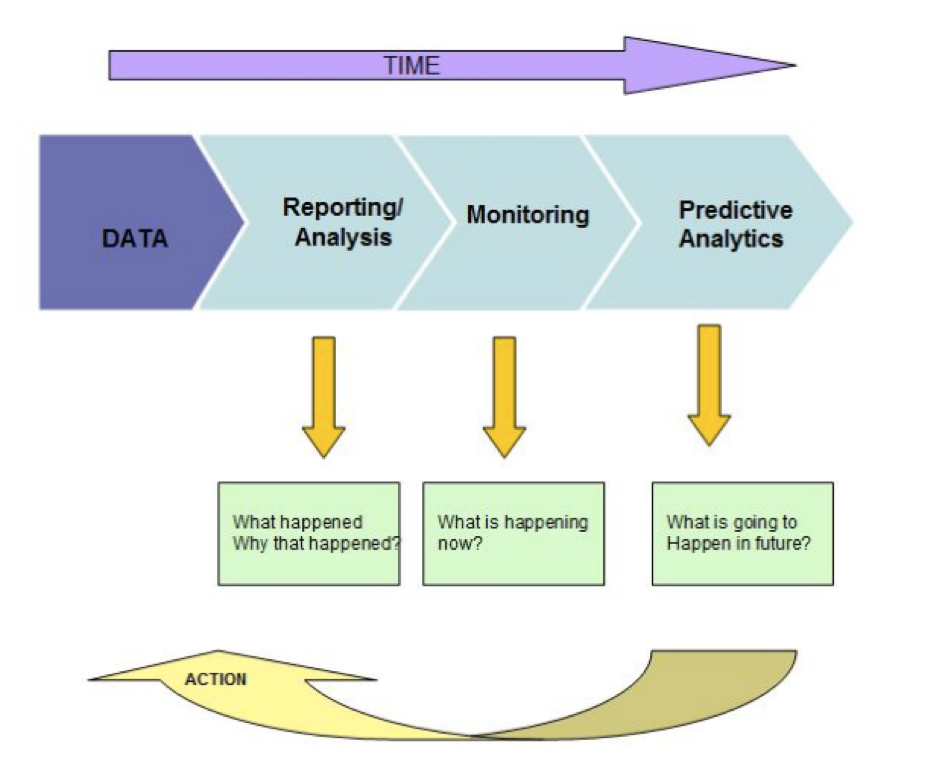
\includegraphics[width=\linewidth]{figures/data_process.png}
  \caption{Процес зміни даних з часом}
  \label{fig:data_process}
\end{figure}

\subsection{Існуючі алгоритми}
Враховуючи те, що результуюча гібридна модель буде використовувати деяку модель в якості базової, доцільно розглянути найбільш поширені алгоритми, що використовуються для класифікації даних. Це дасть змогу зрозуміти головні припципи роботи алгоритмів класифікації, а також за рахунок варіативності даних алгоритмів підкреслити універсальність даного підходу та можливість роботи з будь-якого типу базовими моделями.

\subsubsection{Logistic regression}
В найпростішому випадку опис деякої взаємодії можна звести до двох-трьох категорій змінних за допомогою простих операцій статистики. Проте, в більшості реальних ситуацій потрібно враховувати вплив куди більшої кількості таких змінних, які в загальному випадку можуть бути представлені як багатовимірні таблиці  I × J × K. Саме тому доцільно розглянути узагальнений клас моделей, що носять назву \textit{узагальнених лінійних моделей (\textbf{generalized linear models, GLMs})}. Структурно дані моделі описують шаблони взаємодій та асоціацій. Параметри моделі показують силу таких асоціацій, а основний фокус під час створення таких моделей лягає в оцінку необхідних величин даних параметрів. Узагальнена формула для таких моделей:
\begin{equation}
    \label{eq:logistic_regression}
    y_{i} \sim N(x_{i}^T\beta, \sigma^2)
\end{equation}

Значення вектору $\beta$\ містить коефіцієнти, які і потрібно визначити в ході тренування моделі. В таких моделях значення результуючої змінної підкоряється деякому закону експоненційного розподілу з середнім $\mu_{i}$значенням, який припускається є деякою нелінійною функцією від $x_{i}^T\beta$. Будь-яка модель даного класу містить три основних компоненти:
\begin{itemize}  
	\item Випадковий компонент (\textit{random component}) - відноситься до розподілу ймовірностей результуючої величини $Y$, для лінійної регресії це звичайний нормальний розподіл {Y}. Також носить назву \textit{шуму} або \textit{помилки моделі}.
	\item Систематичний компонент (\textit{systematic component}) - визначає набір додаткових величин $(X_{1}, X_{2}, \ldots X_{k})$ для моделі, а саме їх лінійну комбінацію для створення так званого лінійного провісника (\textit{linear predictor}), наприклад $\beta_{0} + \beta_{1}x_{1} + \beta_{2}x_{2}$ для лінійної регресії.
	\item Зв'язуюча функція (\textit{link function}, $\eta, g(\mu)$) - виражає зв'язок між випадковим та систематичним компонентом. Вона показує, яким чином вихідне значення зв'язане з прогнозованим значенням додаткових величин (наприклад, $\eta = g(E(Y_{i}))=E(Y_{i})$ для лінійної регресії).
\end{itemize}

Загалом серед переваг \textit{GLM}-моделей можна виділити такі:
\begin{itemize}  
	\item не потрібно видозмінювати вихідну величину $Y$, щоб отримати нормальний розподіл;
	\item вибір зв'язуючої функції не залежить від вибору випадкового компоненту, таким чином ми отримуємо більшу гнучкість на етапі моделювання;
	\item якщо зв'язуюча функція адитивна, то нам не потрібно стала дисперсія;
	\item підходи для перевірки моделей є загальними для всіх підвидів класу, тому немає необхідності здійснювати використання окремих інструментів для кожного типу моделі.
\end{itemize}

\subsubsection{Linear Discriminant Analysis}
Linear Discriminant Analysis та Quadratic Discriminant Analysis - два класифікатори, що пропонують лінійну та квадратичну поверхню виборів відповідно. Даного роду алгоритми є досить привабливими, оскільки можуть бути обраховані без додаткових витрат, перевірені на практиці та не мають додаткових метапараметрів для тонкого налаштування.

\begin{figure}[h!]
  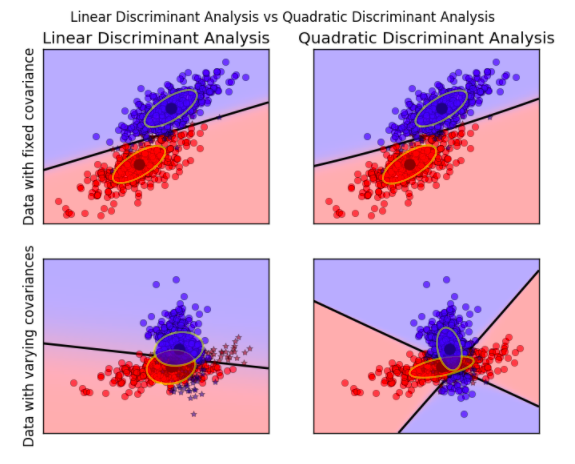
\includegraphics[width=\linewidth]{figures/lda_qda.png}
  \caption{Візуалізація лінійного та квадратичного дискримінантного аналізу}
  \label{fig:lda_qda}
\end{figure}

На рис. \ref{fig:lda_qda} зображено встановлені алгоритмами межі для двох класів. Нижній рядок показує, що лінійний аналіз може здійснити лише лінійний поділ, в той час як квадратичний є більш гнучким. Даний алгоритм часто використовується для зменшення розмірностей простору деякої величини. Він проектує вхідні дані на лінійний підпростір, що максимізує межу поділу між класами. Розмірність вихідних даних завжди менше, ніж кількість класів, тому такий прийом має сенс лише під час виконання мультикласифікації. Обидві моделі унаслідувані від простих ймовірносних моделей на основі умовного розподілу даних $P(X|y  k)$ для кожного класу $k$. Прогнозована величина може бути отримана, використовуючи формулу Байєса:
\begin{equation}
    \label{eq:logistic_regression}
    P(y = k|X) = \frac{P(X|y = k)P(y=k)}{P(X)} = \frac{P(X|y = k)P(y = k)}{\sum_{l}P(X|y=l) \cdot P(y=l)}
\end{equation}

Потім ми обираємо клас $k$, який максимізує умовну ймовірність. Щоб використовувати дану дану модель в якості класифікатора необхідно визначити з вхідних тренувальних даних такі величини: $P(y=k)$ - відношення екземплярів для класу $k$, середні значення для класу $\mu_{i}$ та коваріативну матрицю. У випадку, якщо кількість вхідних даних для тренування досить мала в порівнянні з кількість незалежних змінних датасету (\textit{features}), можна скористатися параметром \textit{усадки} (\textit{shrinkage}). Це значення в межах від 0 до 1, де 1 означає, що діагональна матриця дисперсії буде використана для обрахунку коваріативної матриці. Використання усадки на вхідних даних дає змогу збільшити точність класифікації для варіанту, згаданого вище (рис. \ref{fig:shrinkage}).

\begin{figure}[h!]
  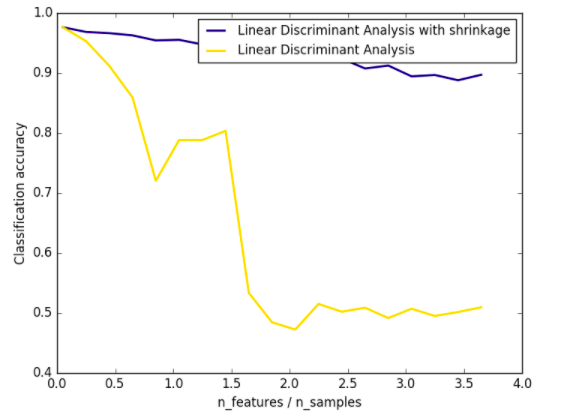
\includegraphics[width=\linewidth]{figures/shrinkage.png}
  \caption{Показники точності з використання усадки та без неї}
  \label{fig:shrinkage}
\end{figure}

\subsubsection{Gaussian Naive Bayes}

\subsubsection{Support Vector machines}

\subsubsection{Decision Tree Classifier}

\subsubsection{K Nearest Neighbours}



\subsection{Оптимізація алгоритмів для використання у предметній галузі}
Оскільки велика кількість алгоритмів вимагають специфічного середовища чи платформи, а для побудови інших необхідні значні обчислювальні потужності, постає проблема платформозалежності та неможливості використання кращих підходів за умови існування додаткових обмежень. Щоб уникнути даних проблем, достатньо розробити рішення, що буде відповідати поставленим нижче вимогам:
\begin{itemize}  
	\item доступ користувача до коду моделі на будь-якій платформонезалежній мові, що дозволить запускати її в довільному середовищі та не спиратися на використання сторонніх бібліотек;
	\item будова моделі та деталі її внутрішньої реалізації повинні бути відкритими, тобто користувач повинен мати змогу переглянути вихідний код і в разі необхідності самостійно відтворити довільний крок та отримати аналогічний результат передбачення для однакового набору вхідних даних;
	\item модель повинна мати точність максимально наближену до точності моделей, що показують найкращі результати для вибраних вхідних даних. Модель повинна мати аналогічні показники щонайменше для 95\% всіх вхідних наборів даних;
	\item виконання коду програми повинно бути швидким (близько 1 мс на рядок вхідних даних).
\end{itemize}

Єдиного рішення, що дозволило б відмовитися від наявних алгоритмів на користь одного, визначеного вимогами вище, поки що немає, але існує підхід, що дозволяє покрити перелік всіх умов. Даний підхід носить назву апроксимаційної моделі [1]. Основна ідея полягає в припущенні, що деяка відносно проста модель, побудована на основі передбачень більш складної моделі може показати схожі результати в межах допустимого відхилення. Саме такою моделлю є RuleFit-модель [2], або модель на основі класу визначених правил. Принцип роботи полягає в серії тренувань дерев вибору на вхідних даних з наступною конвертацією гілок дерев в класи правил. Наприклад, одне правило може виражатися такою формулою: $20 < age <= 30 and income > 10000$. Новий набір даних створюється на основі оригінальних вхідних даних, генеруючи набір індикаторів $0/1$ таким чином, що кожен рядок позначає негативне чи позитивне значення в залежності від результату застосування правила до цього рядка. Дані індикатори потім використовуються в якості значень передбачення для узагальненої лінійної моделі.
\begin{equation}
    \label{eq:linear_model}
    y(w, x) = w_{0} + w_{1}x_{1} + \ldots + w_{p}x_{p}
\end{equation}

Формула \ref{eq:linear_model} описує звичайну модель, що є лінійною комбінацією вхідних значень та вектора коефіцієнтів $w$, а  $y$ – це значення, для якого здійснюється передбачення.

RuleFit є простою моделлю в тому плані, що це лише список правил з відповідними коефіцієнтами для кожного з них. Однак існують і недоліки, пов'язані з тим, що класи правил можуть містити подібні правила, що ускладнює інтуїтивне розуміння впливу коефіцієнтів, тобто вносить складність для розуміння людиною.

Існує дві основних частини в реалізації алгоритму: безпосереднє тренування і передбачення та rulefit задача. Дана задача містить багато параметрів, найголовнішим з яких є альфа-параметр, що визначає розмір регуляризації [3], що застосовується до лінійної моделі RuleFit.

Кінцевим етапом стоврення такої моделі повинна бути валідація згенерованого коду. Оскільки немає жорсткої прив’язки до використовуваної мови, потрібно переконатися, що код компілюється та виконується коректно. Далі потрібно запустити код та зберегти файл з прогнозованими значеннями для подальшого порівняння зі значеннями, що отримуються від оригінальної моделі. Якщо похибка лежить в межах допустимого відхилення валідація вважається успішно пройденою.


\section{Програмна реалізація}
В якості мови програмування було обрано Python, оскільки це високорівнева інтерпретована мова програмування, що дозволяє швидко здійснювати побудову прототипу та скорочує час на розробку продукту вцілому. Значна частина системи являє собою веб-додаток, що стало ще одним фактором під час вибору даної мови, оскільки вона є веб-орієнтованою та містить величезну кількість бібліотек та сторонніх модулів для розробки саме веб-ресурсів. Python також дуже часто використовують в сфері збору та аналізу даних, тому що за рахунок можливості роботи в інтерактивному режимі інтерпретатора можливо значно зекономити час під час роботи з будь-якого роду даними. Гомогенність мов розроблюваних додатків дозволяє зберігати контекст і не перемикатися на синтаксичні відмінності чи особливості мови під час розробки програми. Це, в свою чергу, зменшує час на написання та дозволяє уникнути необхідності працювати з декількома різними мовами одночасно.
\textit{aiohttp} був обраний в якості веб-фреймворку за рахунок своєї асинхронної природи: оскільки основна мета веб-ресурсу коректно обробити вхідні дані від усіх користувачів, потрібно мати змогу асинхронно опрацьовувати велику кількість з'єднань. \textit{Redis} було обрано в якості локальної бази даних за рахунок його швидкодії. Дані зберігаються не на диску, а в пам'яті, що доволяє значно прискорити швидкодію в ситуаціях постійної роботи з записом та читанням. \textit{Redis} також дозволяє здійснювати операцію зберігання поточного стану на диск, тому було також розроблено компонент, що виконує дану діяльність періодично протягом всього часу роботи системи.

\begin{figure}[h!]
  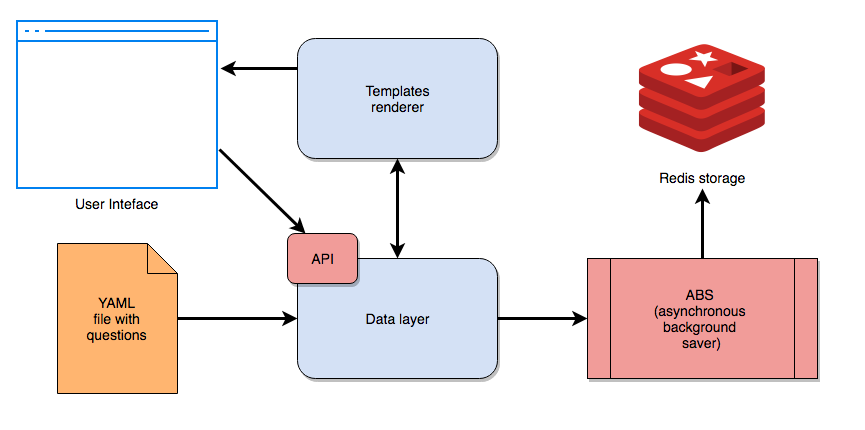
\includegraphics[width=\linewidth]{figures/poll_framework_architecture.png}
  \caption{Гістограма розподілу кількості клієнтів за віком}
  \label{fig:poll_framework_architecture}
\end{figure}

Архітектура мікросервісів була обрана значною мірою тому, що в даному програмному продукті ми маємо окремі повністю незалежні компоненти, які до того ж відповідають за зовсім різні функції системи. Виокремлення системи збору даних дозволяє як і розробляти її окремо та незалежно від інших складових, так і використовувати її в рамках інших систем, а зібрані в результаті її роботи дані в рамках будь-яких інших додатків. Платформа збору даних може бути використана взагалі незалежно в якості платформи для опитування, оскільки була розроблена як фреймворк і відповідно налаштовується під конкретні вимоги користувача. Архітектура фреймворку для опитування зображена на рис. \ref{fig:poll_framework_architecture}.

\subsection{Збір та попередня обробка даних}
Напрямок збору даних розвивався разом з розвитком комунікаційних технологій, а особливо як складова будь-якого бізнес процесу компаній. Проблеми оптимізації систем роботи з клієнтами спричинили появу підходів, які зараз вважаються класичними. В переважній більшості ці підходи покривають 99,9\% поточних бізнес задач. Враховуючи те, що за мету було поставлено не тільки розробку самого алгоритму для побудови моделі, але й збір даних для перевірки роботи цієї моделі, постала потреба загрегувати дані, представити їх у необхідному форматі та обробити їх належним чином. Для роботи з даними була обрана бібліотека \textit{Pandas}, а для роботи безпосередньо з числовими даними, векторами та статистичними функціями - бібліотека \textit{NumPy}. Серед науковців та спеціалістів з обробки даних також широко використовується мова програмування \textit{R}, яка уже містить значну частину вбудованих методів та навіть засобів візуалізації в стандарнтій бібліотеці самої мови, та \textit{Python} був обраний з урахуванням необхідності розробки всього програмного комплексу в рамках однієї мови програмування.

Процес обробки даних, трансформації значень та представлення даних в узагальненому форматі можна зобразити у вигляді діаграми на рис. \ref{fig:data_processing}

\begin{figure}[h!]
  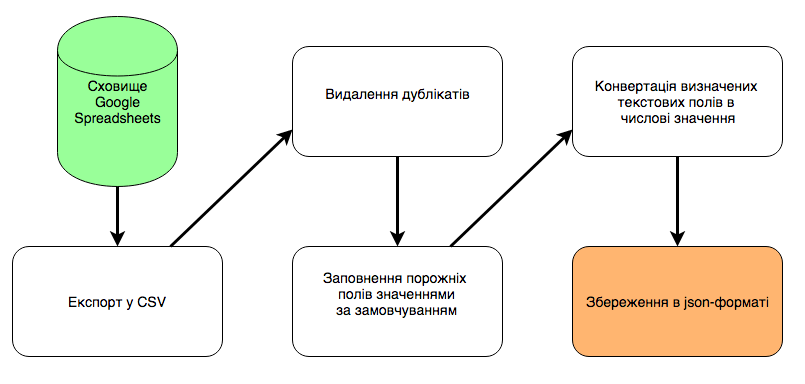
\includegraphics[width=\linewidth]{figures/data_processing.png}
  \caption{Етапи попередньої обробки даних}
  \label{fig:data_processing}
\end{figure}

В кінцевому результаті дані зберігаються в уніфікованому \textit{json}-форматі, що дає змогу: використовувати їх безпосередньо в консолі браузера для простішого перегляду і відлагодження; проводити легку конвертацію в \textit{csv}-формат, який очікує більшість інструментів з обробки даних; перетворювати їх в \textit{Python}-об'єкти для роботи з ними в коді програми; передавати на обробку в інші методи та функції, що вже готові працювати з даним форматом без необхідності додаткових серіалізацій/десеріалізацій; здійснювати конвертацію цих даних з додаванням відношень і зв'язків між ними (наприклад, для зберігання в реляційній \textit{SQL}-базі даних); зберігати на диск з можливістю перегляду в будь-якому текстовому редакторі.

Перед етапом обробки даних та жорсткого втручання в них (видалення записів, модифікація існуючих значень, заміна чи конвертація полів) необхідно мати загальне уявлення про вміст та загальні характеристики даних. На даному етапі на допомогу приходить статистика та її методи.
\textit{Статистика} - за своїм строгим визначенням не є технологією збору даних, проте саме вона використовується задля того, що знайти закономірності в даних та для наступної побудови прогностичних моделей. Також, з точки зору користувача, ви завжди будете стикатися з тими чи іншими інструментами статистики в будь-яких інших методах збору та аналізу даних. Статистика загалом являє собою розділ математики, пов'язаний зі збором та описом даних. Статистика займається підрахунком ключових значень та ймовірностей. Використання її в процесі збору даних допомагає відповісти на ряд важливих запитань, що відносяться до ваших даних: які закономірності прослідковуються з базі даних; яка ймовірність того, що обрана подія настане; які закономірності найбільш важливі; яку загальну інформацію можна отримати про дані, щоб зрозуміти з якого роду значеннями ми маємо справу.

Дану інформацію надалі можна використовувати для роботи з даними, оскільки це свого роду надає додаткову інформацію про доменну область (наприклад, на рис. зображена гістограма, що дає змогу швидко встановити факт про вік переважної кількості цільової аудиторії: більше 50). Інші з найчастіше вживаних метрик статистики:
\begin{itemize}
	\item \textit{max} - максимальне значення цільової величини;
	\item \textit{min} - мінімальне значення цільової величини;
	\item \textit{mean} - середнє значення обраної величини;
	\item \textit{median} - значення, що розділяє вибірку на дві підмножини з максимально наближеної кількістю елементів у кожній;
	\item \textit{mode} - значення, що зустрічається найчастіше;
	\item \textit{variance} - показник відхилення цільового значення від середнього у вибірці.
\end{itemize}

\begin{figure}[h!]
  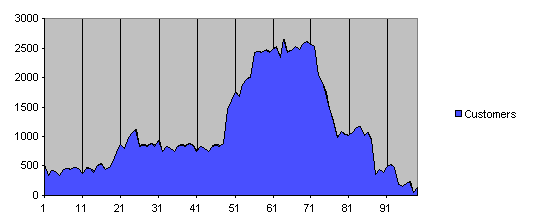
\includegraphics[width=\linewidth]{figures/statistics.png}
  \caption{Гістограма розподілу кількості клієнтів за віком}
  \label{fig:statistics}
\end{figure}

Останній показник, дисперсія, дещо складніший для розуміння: чим вище значення, тим більш дані різнорідні і різняться між собою. Якщо ж значення менше - дані загалом схожі і мало відрізняються від середнього по вибірці. Базуючись на статистичних даних, користувач має змогу налаштувати модель таким чином, щоб передбачуване значення максимально відоражало реальну зміну величини.

Для збору даних та формування початкового датасету було створено допоміжний додаток у вигляді веб-ресурсу. Він являє собою веб-сайт, на якому здійснюються опитування серед різних класів респондентів: студентів, випускників та викладачів. Кожен учасник опитування заповнює невелику тематичну анкету, на основі якої формуюється таблиця вхідних даних. Загальну архітектуру додатку можна побачити на рис. \ref{fig:poll_architecture} 

\begin{figure}[h!]
  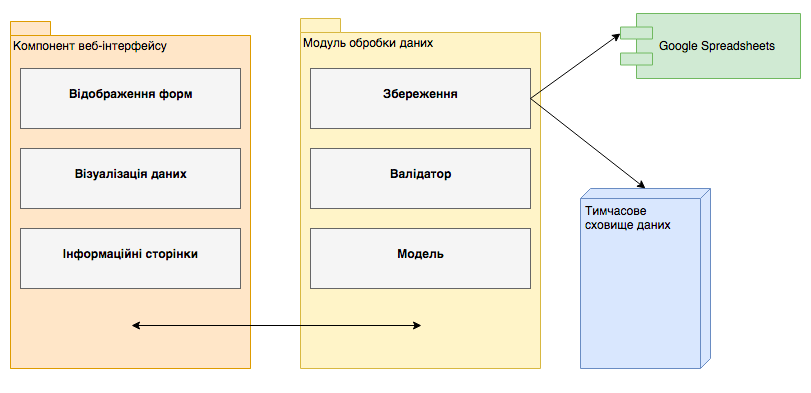
\includegraphics[width=\linewidth]{figures/poll_architecture.png}
  \caption{Загальна архітектура додатку опитування}
  \label{fig:poll_architecture}
\end{figure}

Система побудована на основі архітектури мікросервісів і дотримання принципу делегування частини роботи зовнішнім ресурсам. За рахунок такого підходу можна отримати більшу ефективність, стабільність та пропускну здатність роботи системи, але знижується надійність, оскільки вихід хоча б одного компоненту з ладу призведе до повної недієздатності системи. Враховуючи важливий фактор роботи з даними, потрібно розуміти, що втрати на етапі збору значно впливають на подальші результати. Саме тому було додамо внутрішнє тимчасове сховище даних, яке слугує для збереження резервних копій. Система складається з таких компонентів:
\begin{itemize}
	\item Веб-інтерфейс - являє собою веб-додаток, що побудований на основі aiohttp веб-фреймоврку та здійснює основні функції обробки користувацької логіки. Він відповідає за рендеринг сторінок, видачу статичних ресурсів, обробку та роутинг запитів та спілкується з іншими компонентами для подальшоої передачі даних. 
	\begin{itemize}
		\item Відображення форм - підкомпонент, що відповідає за відображення користувацького інтерфейсу та безпосередню взаємодію з користувачем за допомогою веб-браузера.
		\item Візуалізація даних - представлення вхідних, існуючих, а також відображення статусу обробки поточних даних для розуміння стану даних та прогресу під час заповнення форми опитування.
		\item Інформаційні сторінки - відображення статичних сторінок веб-ресурсу для надання додаткової інформації та для отримання зворотного зв'язку.
	\end{itemize}
	\item Модуль обробки даних - здійснює фільтрацію, нормалізацію та перетворення даних таким чином, щоб вони були уніфікованого формату та могли бути використанні надалі іншими компонентами. Обробка здійснюється з використанням можливостей самої мови, а також з допомогою сторонніх бібліотек \textit{NumPy} та \textit{Pandas}.
	\begin{itemize}
		\item Підкомпонент збереження даних - створення об'єктів для кінцевих даних форм на основі моделей; створення асинхронних задач збереження даних; переріодична інкрементальна відправка проміжного стану для формування єдиної бази, використовуючи сторонній сервіс \textit{Google Spreadsheets}. Збереження виконується як локально, використовуючи базу даних в оперативній пам'яті, так і віддалено, використовуючи основну базу даних на основі таблиць.
		\item Валідатор - здійснення перевірки даних на коректність та відповідність вхідним обмеженням. Видача повідомлень про помилку в разі невідповідності.
		\item Модель - \textit{data access object}, представлення вхідних даних у вигляді об'єктів мови програмування для надання зручного доступу до даних з коду програми. Серіалізація моделі дозволяє зберегти дані для подальшого використання та можливої додаткової обробки. За допомогою формального представлення даних у вигляді моделі можливо з легкістю проводити маніпуляції з даними в рамках інструментів мови програмування.
	\end{itemize}
\end{itemize}

Особливості даних можна встановити ще на етапі їх збору. Навіть не здійснюючи жодного аналізу чи попередньої обробки можливо отримати деякі важливі характеристики даних або просто візуалізувати їх для зручнішого сприйняття чи для кращого усвідомлення того, з якого роду даними доведеться працювати. Саме для таких цілей і використовується \textit{exploratory data analysis} - аналіз даних з метою попереднього дослідження вхідних даних.

Візуалізація даних загалом здійснюється для таких цілей:
\begin{itemize}  
	\item Комунікативна складова:
	\begin{itemize}
		\item представити дані та ідеї;
		\item проінформувати;
		\item підтримати і аргументувати;
		\item вплинути і переконати;
	\end{itemize}
	\item Дослідницька:
	\begin{itemize}
		\item вивчити (дослідити) дані;
		\item проаналізувати ситуацію;
		\item визначити наступні кроки;
		\item прийняти рішення стосовно деякого питання;
	\end{itemize}
\end{itemize}

Оскільки одним із компонентів збору даних був \text{Google Spreadsheets}, то початкова візуалізація даних не становила жодної складності, тому що даний ресурс містить вбудовані засоби для цього рис. \ref{fig:answer_visualize} 

\begin{figure}[h!]
  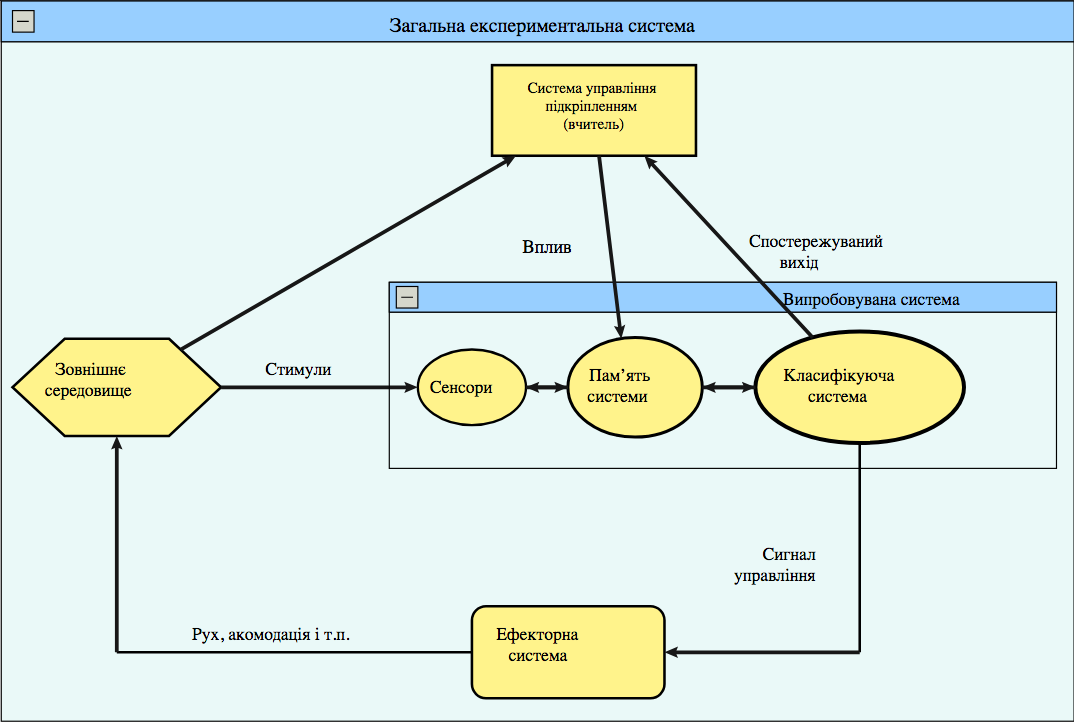
\includegraphics[width=\linewidth]{figures/fig_system.png}
  \caption{Візуалізація відповідей однієї з форм анкети опитування}
  \label{fig:answer_visualize}
\end{figure}

Для збору даних потрібно враховувати декілька важливих нюансів. По-перше, це \textit{робота з неповними даними} - ситуація, коли зібрані дані не віповідають поставленим критеріям чи не проходять валідацію, але не можуть бути відкинуті, оскільки є досить важливими. Схожа ситуація може відбутися, коли дані взагалі зберігаються в різної кількості форматах та структур, тому виділити один загальний критерій для валідації може бути досить важко. Тому потрібно завжди враховувати випадок обробки та роботи з неповними даними. 

\textit{Врахування ефективності алгоритмів, що використовуютьс з роботи з даними} - під час обробки невеликої кількості даних ефективність алгоритму не відіграє значної ролі, оскільки обчислювальних ресурсів комп'ютера зазвичай більш ніж досить, тому користувач майже не помічає затримок у роботі. Але з ростом об'єму даних (які можуть сягати декількох сот гігабайт) час на їх обробку може зростати нелінійно, а отже операції можуть перевищувати встановлені обмеження на тривалість роботи. Тому необхідно враховувати кількість даних, з якими повинна буде працювати системи і обирати максимально ефективні алгоритми для роботи.

\textit{Отримання великого обсягу початкових даних} - під час скрапінгу веб-ресурсів або під час потокового отримання вхідних даних (\textit{streaming}) можуть виникнути проблеми, пов'язані з неможливістю процесу обробити всі дані одночасно чи зберігати їх в рамках однієї сесії в оперативній пам'яті. Для вирішення такої проблеми можна скористатися такими підходами: кешування інформації на проміжних етапах, використання вбудованих функцій замість написання власних послідовностей обробки на стороні бізнес-логіки (прикладом може бути використання stored procedures під час роботи з \textit{SQL} базами даних), побудова алгоритмів, що використовують принцип \textit{pipeline} (вихід одніє функції відразу слугує вхідними даними для іншої, таким чином відпадає необхідність зберігати дані в проміжному стані та витрачати додатковий простір на жорсткому диску), пакетна обробка даних.

\textit{Обробка даних, що містять зв'язки між собою} - досить поширена ситуація, коли одні дані містять посилання на інші, або потрібно відслідковувати зв'язки між певними компонентами вхідної інформації. В такому випадку немає простих рішень чи рекомендації, оскільки в будь-якому випадку потрібно буде підтримувати структуру даних, що буде відповідати за збереження даних зв'язків. Очевидним рішенням є використання реляційних баз даних, які будуть підтримувати структуру і відношення чи альтернативне використання графових баз даних, принцип яких саме в побудові бази таким чином, щоб вона представляла собою граф відносин між даними.

\textit{Обробка даних, що містять зв'язки між собою} - досить поширена ситуація, коли одні дані містять посилання на інші, або потрібно відслідковувати зв'язки між певними компонентами вхідної інформації. В такому випадку немає простих рішень чи рекомендації, оскільки в будь-якому випадку потрібно буде підтримувати структуру даних, що буде відповідати за збереження даних зв'язків. Очевидним рішенням є використання реляційних баз даних, які будуть підтримувати структуру і відношення чи альтернативне використання графових баз даних, принцип яких саме в побудові бази таким чином, щоб вона представляла собою граф відносин між даними.

\textit{Підтримка гетерогенності джерел інформації} - системи, що використовуються для отримання даних можуть не мати уніфікованого інтерфейсу та не надавати однакові можливості зі свого боку для здійснення запитів. Потрібно враховувати відмінності між кожним окремим джерелом, а також розуміти встановлені обмеження (наприклад, багато веб-ресурсів встановлюють обмеження на кількість запитів, що здійснюються за певний проміжок часу). Тому якщо додаток буде розроблено без урахування таких відмінностей - він може показати добрі результати під час роботи з одним провайдером інформації, але для інших він не буде функціонувати належним чином.


\subsection{Побудова моделі}
Для створення ефективної кінцевої моделі розроблюваний алгоритм повинен підповідати таким вимогам:
\begin{itemize}  
	\item відкритий доступ користувача до коду моделі на будь-якій платформонезалежній мові, що дозволить запускати її в довільному середовищі та не опиратися на використання сторонніх бібліотек;
	\item будова моделі та деталі її внутрішньої реалізації повинні бути відкритими, тобто користувач повинен мати змогу переглянути вихідний код і в разі необхідності самостійно відтворити довільний крок та отримати аналогічний результат передбачення для однакового набору вхідних даних;
	\item модель повинна мати точність максимально наближену до точності моделей, що показують найкращі результати для вибраних вхідних даних. Модель повинна мати аналогічні показники щонайменше для 95\% всіх вхідних наборів даних;
	\item виконання коду програми повинно бути швидким (близько 1 мс на рядок вхідних даних).
\end{itemize}

\subsection{Висновки розділу?}
Результати показують, що стабільно показують чудові результати для завдань класифікації
текстів, суттєво перевищуючи показники інших методів.
\section{Аналіз рішення}
 Анализ, согласно критериям как работает, пути улучшения (таблица сравнения с существующими подходами, графики, диаграммы)

\subsection{Порівняльний аналіз}
Було проведено порівняльний аналіз рішення з існуючими реалізаціями для підтердження ефективності використання даного алгоритму. Обрані такі критерії для побудови порівняльної таблиці:

\begin{itemize}
	\item відхилення від еталонної величини;
	\item середнє квадратичне відхилення
	\item Підтверджено значно більші показники швидкодії моделі, розробленої за допомогою даного підходу.
\end{itemize}


Також для найкращої моделі та гібридної моделей були побудовані таблиці помилок (\textit{confusion matrix}) - матриці, що допомагають візуалізувати ефективність алгоритмів. Кожна колонка містить кількість результатів в передбачуваному класі, в той час як кожен рядок містить дійсну кількість елементів у класі (рис. \ref{fig:confusion_matrix}).

\begin{figure}[h!]
  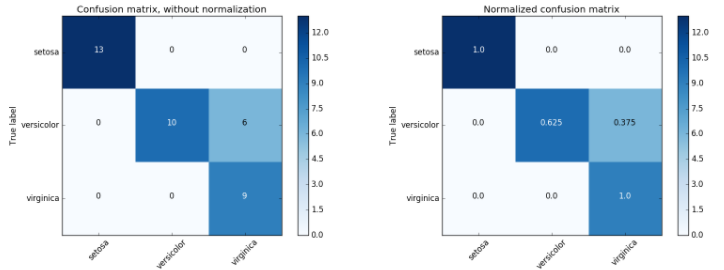
\includegraphics[width=\linewidth]{figures/confusion_matrix.png}
  \caption{Приклад матриці помилок для вхідного набору даних Iris}
  \label{fig:confusion_matrix}
\end{figure}

Результати для моделі \textit{Support Vector Machines} та побудованої гідбридної моделі (табл. \ref{tab:confusion_matrix}) дають змогу зрозуміти, обидві моделі відносять елементи до однакових класів. Це означає, що хоч і точніть передбачення не є максимально можливою, проте дозволяє показати стабільні консистенті результати для обох моделей, а це, у свою чергу, дозволяє підтверджувати надійність розроблюваного підходу.

\begin{table}[h!]
	\begin{tabularx}{\textwidth}{|X|X|X|X|}
    \hline
     & setosa & versicolor & virginica \\ \hline
    setosa & 7 & 0 & 0 \\ \hline
    versicolor & 0 & 10 & 2 \\ \hline
    virginica & 0 & 0 & 11 \\
    \hline
    \end{tabularx}
\caption{Матриця помилок} \label{tab:confusion_matrix}
\end{table}

Швидкодія роботи на різних вхідних даних
 \subsection{Отримані результати та шляхи покращення}
 Отже, в результаті отримана реалізація показала відповідність усім висунутим вимогам та продемонструвала стабільні показники незалежно від виду та об'єму вхідних даних. На поточному етапі такі результати повністю задоволняють як користувачів алгоритму, так і розробників, які бажають покращити алгоритм чи модифікувати його будь-яким чином для забезпечення кращих показників точності чи швидкодії.

Серед напрямків для покращення алгоритму можна виділити такі основні:

\begin{itemize}
	\item Визначення оптимального алгоритму не шляхом повного перебору існуючих моделей, а за допомогою деякої евристики. Зараз для вхідних даних необхідно побудувати всі моделі, користуючись медотом повного перебору () і виконати їхнє порівняння за деякою обраною метрикою. Лише після цього на основі кращої моделі буде побудована наша гібридна модель. Якщо ж скористатися деяким набором правил, евристикою чи іншими додатковими знаннями в доменній залузі - можна обмежити кількість моделей, що будуть побудовані, таким чином в декілька разів зменшити витрати на час на етапі побудови моделей. Виграш буде значно відчутний на великій кількості моделей за умови, що лише кілька з них дійсно показують стабільно найкращі результати для схожих вхідних даних. Однією із можливих реалізацій такого прийому може бути додаткова модель-класифікатор, що буде на основі вхідних даних обирати клас алгоритмів (деяке значення Т), для яких варто проводити побудову моделей. Іншим варіантом може бути підтримка структури у вигляді словника, що буде зберігати наперед визначені користувачем набори типу "критерій"-"клас алгоритмів" і значно швидше (за лінійний час) буде обирати потрібну множину алгоритмів. Останній підхід є значно швидшим, але вимагає додаткової початкової ініціалізації та втручання людини для підготовки такого словника.
	\item Запуск побудови кожної моделі в окремому потоці. Процес побудови моделі є процесом, що в першу чергу вимагає процесорний час для виконання (\textit{cpu-bound}), тому з апаратної точки зору прискорити його роботу можливо за рахунок розпаралелювання на декількох ядрах процесора. Найпростішим варіантом є використання багатоядерних процесорів і виконнання алгоритму на окремому ядрі. Сучасні відеокарти з підтримкою технологій \textit{Nvidia CUDA} та \textit{AMD OpenCL} теж можуть бути використані для запуску даних алгоритмів. Порівняння показують, що використання відеокарт для схожих обрахунків може надати приріст у розмірі 90-95х кратного прискорення роботи. Аналогічним чином можна скористатися розподіленими та багатопроцесрними системами, коли алгоритми будуть виконуватися окреми на різних машинах в межах одного кластеру. Головним недоліком таких систем є підвищення порогу входження для розробки, адже це вимагає додаткових знань як для написання коду (\textit{C++, MPI, OpenMPI}), так і розуміння архітектури розподілених систем вцілому. Наприклад, для написання алгоритму для кластеру потрібно розуміти, що кожна модель на окремій ноді кластеру повинна мати доступ до вхідного датасету, а отже потрібно забезпечити централізований неблокуючий доступ до даних або реалізувати можливість спільної пам'яті (\textit{shared memory}), що теж вимагає додаткових зусиль з точки зору програміста. З переваг варто відмітити однократність даної операції та практично необмежений лінійний ріст ефективності пропорційно до кількості початкових алгоритмів.
	\item Під час сумісної роботи над проектом виникає необхідність обміну даними між розробниками. Науковці хочуть мати змогу надсилати моделі іншим, а також мати змогу їх зберегти для подальшого використання. Тому ще одним можливим шляхом для вдосконалення може бути можливість серіалізації моделей. Таким чином модель можна буде побудувати і зберегти в бінарному форматі на одному комп'ютері, а потім використати в майбутньому без необхідності повторної її перебудови. Звісно такий підхід працює лише для одного набору вхідних даних, тому область його застосування досить обмежена. Проте, якщо над деякими даними працює команда науковців, саме це дасть змогу швидко обмінюватися результатами чи використовувати напрацювання інших. Найпростішою реалізаціює тут може бути знімок об'єкта у пам'яті, але таким чином втрачається кросплатформенність та машинонезалежність. Вбудовані підходи до серіалізації (наприклад, \textit{pickle}) також будуть страждати від подібних нюансів. Саме тому необхідно буде розробити додатковий алгоритм для серіалізації моделей, що і є головним фактором, який стримує додавання даної можливості до існуючого коду.
\end{itemize}

Розглянуті напрямки покращення дозволять збільшити швидкодію програми вцілому, а також спростити використання її в межах команди науковців, а тому доцільно розглянути подальшу роботу над проектом саме в одному із запропонованих напрямків.
\section{Стартап}
Для впровадження продукту в якості стартапу потрібно виділити основну інноваційну складову, яка і буде позиціонувати продукт на ринку та визначати його нішу серед конкурентів. Такою складовою є компонент, що безпосередньо відповідає за побудову моделі та здійснення прогнозування. Саме тому надалі порівняння і критерії будуть виділені лише для цього окремого компоненту.

\begin{table}[h!]
\fontsize{12pt}{12pt}\selectfont
	\begin{tabularx}{\textwidth}{|X|X|X|}
	\hline
	Зміст ідеї & Напрямки застовування & Вигоди для користувача \\ \hline
	\multirow{3}{*}{Система побудови універсальних прогностичних моделей та метод для додавання  нових алгоритмів в дане рішення} & 1. Використання науковцями та спеціалістами з аналізу даних для підвищення їх ефективності та продуктивності роботи загалом & Зручний та зрозумілий вихідний код дозволить працювати значно ефективніше, тим самим зосереджуючись на прикладних задачах, замість деталей реалізації \\ \hline
	2. Узагальнення алгоритмів для роботи з різними типами даних & Універсальність моделі дозволить не перемикати контексти під час роботи з різними типами даних, використовуючи однаковий підхід для вхідної інформації \\ \hline
	3. Отримання кращих результатів передбачень для даних, що змінюються з часом & Допомога під час роботи з величинами, що залежать від часу: курси валют, показники біржі, зміни клімату \\
	\hline
	\end{tabularx}
\caption{Опис ідеї стартап-проекту} \label{tab:stab_0}
\end{table}

Маркетингова діяльність повинна починатися з дослідження макросередовища, вивчення ринку в цілому. Основні категорії, які виділяють для такого роду досліджень: показники виробництва, які характеризують пропозицію товарів; показники, що характеризують попит на товари; показники які характеризують ринкові ціни. Дослідження дало змогу сформувати дані показники в стислій формі таблиці, що відображено на табл. \ref{tab:stab_1}.

\begin{table}[h!]
\fontsize{12pt}{12pt}\selectfont
	\begin{tabularx}{\textwidth}{|c|X|X|}
    \hline
    № п/п & Показники стану ринку (найменування) & Характеристика \\ \hline
    1 & Кількість головних гравців, од & 1 \\ \hline
    2 & Загальний обсяг продаж, грн/ум. од & 914 218 млн грн \\ \hline
    3 & Динаміка ринку (якісна оцінка) & Спадає \\ \hline
    4 & Наявність обмежень для входу (вказати характер обмежень) & Висока доля невизначеності, відсутність попереднього досвіду та необхідних статистичних даних \\ \hline
    5 & Специфічні вимоги до стандартизації та сертифікації & - \\ \hline
    6 & Середня норма рентабельності в галузі (або по ринку), \% & 18-20\% \\
    \hline
    \end{tabularx}
\caption{Попередня характеристика потенційного ринку стартап-проекту} \label{tab:stab_1}
\end{table}

Ринок є доволі привабливим для входження: пристойна середня норма рентабельності, що трохи вищ аза середній банківський відсоток на вклади у гривні, а спадання ринку потенційно відкриває його для нестандартних інноваційних рішень, оскільки існує дуже висока необхідність в розробці універсального методу для відновлення зображень.

\begin{table}[h!]
\fontsize{12pt}{12pt}\selectfont
	\begin{tabularx}{\textwidth}{|c|X|X|X|X|}
    \hline
    № п/п & Потреба, що формує ринок & Цільова аудиторія (цільові сегменти ринку) & Відмінності у поведінці різних потенційних цільових груп клієнтів & Вимоги споживачів до товару \\ \hline
    1 & Необхідність для інвесторів знайти перспективний метод для вкладень & Люди, які мають фінансову можливість та зацікавленість робоити інвестиції у інноваційні проекти & Люди, які мають фінансову можливість та зацікавленість робити інвестиції у інноваційні проекти мають на меті збільшення свого капіталу, підвищення свого іміджу, а також долучитися до новітніх технологій, щоб бути у тренді & Необхідно розробити методику оцінювання та рекомендації, які б з високою ймовірністю розраховували потенційні необхідні інвестиції та шляхи попередження ключиових ризиків \\ \hline
    2 & Необхідність команди для побудови цього & Активні люди, які бажають втілити у життя свій проект & Необхідність проаналізувати всі ключові фактори, щоб визначити, чи доцільно реалізовувати проект та чи вдасться залучити спонсорів & Високоточний метод оцінки відновлення зображень, щоб визначити доцільність реалізації відновлення зображень \\
    \hline
    \end{tabularx}
\caption{Характеристика потенційних клієнтів стаптап-проекту} \label{tab:stab_2}
\end{table}

Для того, щоб успішно виживати в довгостроковій перспективі, підприємство повинно вміти передбачати, які саме труднощі можуть виникнути на його шляху в майбутньому і які нові можливості можуть відкритися для нього. Тому аналіз повинен враховувати влив факторів на окремі складові продукту та підприємства в цілому.

\begin{table}[h!]
\fontsize{12pt}{12pt}\selectfont
	\begin{tabularx}{\textwidth}{|c|X|X|X|}
    \hline
    № п/п & Фактор & Зміст загрози & Можлива реакція компанії \\ \hline
    1 & Попит & Не вдасться розробити унікальний метод, який би можна було застосовувати для будь-яких алгоритмів та адаптувати для роботи з різними типами даних & Розробка максимально універсального методу \\ \hline 
    2 & Конкуренція & Можливість появи конкурентів з дуже схожими функціями, їх вихід на ринок раніше за нас & Доопрацювання якості розроблюваного методу з фокусом на зручність та простоту використання, розробка нових властивостей, яких немає у конкурента. Розгляд можливості об'єднання компаній для подальної спільної роботи. \\ \hline 
    3 & Економічні & Зменшення доходу інвесторів, що призведе до зменшення кількості інвестицій & Моніторинг економічної ситуації у країні, пошук закордонних користувачів та адаптація для світового ринку \\
    \hline
    \end{tabularx}
\caption{Фактори загроз} \label{tab:stab_3}
\end{table}

Ринкові можливості - це сприятливі обставини, які підприємство може використовувати для отримання переваг. Погіршення позицій конкурентів, різке зростання попиту, поява нових технологій, зростання рівнів доходів населення - це все можливості для проекту, які слід використовувати.

\begin{table}[h!]
\fontsize{12pt}{12pt}\selectfont
	\begin{tabularx}{\textwidth}{|c|X|X|X|}
    \hline
    № п/п & Фактор & Зміст можливості & Можлива реакція компанії \\ \hline
    1 & Попит & Унікальність пропонованого функціоналу та додаткових можливостей при умові невисокої конкуренції дозволить захопити велику частку ринку, особливо зацікавивши додатком невеликих інвесторів (бізнес-ангелів) та команди проектів, які не потребують значних інвестицій & Адаптація до ринку, що розширяється, моніторинг новітніх розробок та ризиків, які тіьки нещодавно з'явилися \\ \hline
    2 & Науково-технічні & Поява нових технологій, виникнення нових ринкових умов та факторів, які виявлять значний вплив на розвиток алгоритмів класифікації  & Активне використання використання рішення; у випадку, якщо наше рішення буде адним з перших та матиме суттєві відмінності від аналогів, захист інтелектуальної власності розробників, патентування цієї технології та додання її до інтелектувальних активів проекту \\ \hline
    3 & Соціально-культурні & Велика популярність сфери роботи з даними та їх аналізу & Адаптація системи до розширення ринку, появи нових умов та технологій \\
    \hline
    \end{tabularx}
\caption{Фактори можливостей} \label{tab:stab_3}
\end{table}

Ступеневий аналіз виконується у вигляді таблиці, що описує динаміку розвитку конкурентного середовища та головних гравців ринку. Дані критерії (табл. \ref{tab:stab_4_1}) дозволють оцінити головних конкурентів на ринку за виділеними основними критеріями, що характеризують їх з різних економічних точок зору.

\begin{table}[h!]
\fontsize{12pt}{12pt}\selectfont
	\begin{tabularx}{\textwidth}{|X|X|X|}
    \hline
    Особливості конкурентного середовища & В чому проявляється дана характеристика & Вплив на діяльність підприємства (можливі дії компанії, щоб бути конкурентноспроможною) \\ \hline
    1. Тип конкуренції - чиста конкуренція & Велика кількість методів відновлення зображень, частина з яких є запатентованою інтелектувальною власністю & Звертати увагу на якість та універсальність методу відновлення зображень \\ \hline 
    2. За рівнем конкурентної боротьби - національний & Відновлення зображень не буде прив'язуватися до географічних показників & Акцент в рекламі на потреби жителів великих міст (столиці), таргетування на науковців та молодих дослідників, а також на високозабезпечених людей - потенційних інвесторів \\ \hline 
    3. За галузевою ознакою - внутрішньогалузева & Конкуренцію складають подібні методики розробки прогностичних моделей & Акцентувати увагу на незвичайність подачі послуг, а також зручність у використанні та надійність, яку вони забезпечують \\
    \hline
    \end{tabularx}
\caption{Ступеневий аналіз конкуренції на ринку} \label{tab:stab_4_1}
\end{table}

\begin{table}[h!]
\fontsize{12pt}{12pt}\selectfont
    \begin{tabularx}{\textwidth}{|X|X|X|}
    \hline
    \textit{Особливості конкурентного середовища} & \textit{В чому проявляється дана характеристика} & \textit{Вплив на діяльність підприємства (можливі дії компанії, щоб бути конкурентноспроможною)} \\ \hline
    4. Конкуренція за видами товарів - між бажаннями & Потенційні клієнти роблять вибір між звичними методами побудови моделей (яких дуже велика кількість) і відчувають складність у виборі найбільш доцільного методу & Чітко зрозуміти потреби та бажання кожної з груп цільової аудиторії та розробляти гнучку систему, яка задовольнятиме потреби всіх груп користувачів \\ \hline 
    5. За характером конкурентних переваг - нецінова & Акцент знаходиться на унікальності та якості послуг, що надаються, а також на перевагах, які отримує клієнт під час використання наших послуг & Робота над покращення методики побудови прогностичних моделей та підвищенням її універсальності \\ \hline 
    6. За інтенсивністю - не марочна & Продається втілення ідеї, а не певний бренд & Просування ідеї у соціальних мережах \\
    \hline
    \end{tabularx}
\caption{Ступеневий аналіз конкуренції на ринку (продовження)} \label{tab:stab_4_2}
\end{table}

Особливості конкурентного середовища дають змогу краще зрозуміти, з якого плану умовами та якого роду аналогами доведеться зіткнутися продукту під час боротьби за частку ринку.

\begin{table}[h!]
\fontsize{12pt}{12pt}\selectfont
	\begin{tabularx}{\textwidth}{|X|X|X|X|X|X|}
    \hline
    Складові аналізу & Прямі конкуренти в галузі & Потенційні конкуренти & Постачальники & Клієнти & Товари-замінники \\ \hline
     & Прямих конкурентів немає, непрямі - різноманітні методи побудови прогностичних моделей & Нові розробки у галузі & Інвестори диктують умови розвитку ринку: ключова умова - проект повинен бути потрібним користувачам та приносити користь & Кількість зацікавлених клієнтів, рівень зацікавленості в такому типі послуг & Поява схожих дешевших або якісніших продуктів-конкурентів \\ \hline
    Висновки & Прямих конкурентів немає & - можливості входу в ринок присутні, необхідно вирішити проблему пошуку та адаптації статистичних даних - необхідність розробки універсального методу, який може бути використаний як інвесторами, так і командою проекту & Успіх нашого проекту залежить від рівня довіри інвесторів та команд проекту до новітнього методу побудови прогрностичних моделей & Клієнти формують попит на таку послугу & Універсальних методів, які могли б замінити запропонований проект немає \\
    \hline
    \end{tabularx}
\caption{Аналіз конкуренції в галузі за М. Портером} \label{tab:stab_5}
\end{table}

Розроблена Майклом Портером методика для аналізу галузей і вироблення стратегії бізнесу дозволяє оцінити привабливість ведення бізнесу в конкретній галузі, виділяючи п'ять сил, які визначають рівень конкуренції. Привабливість в даному контексті має на увазі рентабельність галузі, тобто найпривабливішою є галузь, що наближається до досконалої конкуренції (\ref{tab:stab_5}. Виділяють п'ять основних сил: аналіз загрози появи продуктів-замінників; аналіз загрози появи нових гравців; аналіз ринкової влади постачальників; аналіз ринкової влади споживачів; аналіз рівня конкурентної боротьби.

\begin{table}[h!]
\fontsize{12pt}{12pt}\selectfont
	\begin{tabularx}{\textwidth}{|l|X|X|}
    \hline
    № п/п & Фактор конкурентноспроможності & Обгрунтування (наведення чинників, що роблять фактор для порівнянння конкурентних проектів значущим) \\ \hline
    1 & Фактор часу & Ідея є частково новою, для перейняття ідеї та втілення її у життя потенційним конкурентам знадобиться час \\ \hline
    2 & Фактор новизни товару & Початковий успіх продукту очікується через його новизну та інтерес цільової аудиторії до нових інноваційних рішень \\ \hline
    3 & Фактор якості послуг та надання інформації & Науковці та експерти з обробки даних потребують універсальний метод побудови прогностичних моделей \\
    \hline
    \end{tabularx}
\caption{Обґрунтування факторів конкурентноспроможності} \label{tab:stab_6}
\end{table}

Аналіз внутрішніх сильних і слабких сторін рекомендується проводити як порівняльний аналіз, причому головний напрям уваги має спрямовуватися на конкурентноспроможність продукту. Критерії, які повинні оцінюватися охоплюють цілу низку показників, до основних груп яких входять: прибутковість; репутація; продуктивність; асортимент; впровадження іновацій.

\begin{table}[h!]
\fontsize{12pt}{12pt}\selectfont
	\begin{tabularx}{\textwidth}{|l|X|X|X|X|X|X|X|}
    \hline
    № п/п & Фактор конкурентноспроможності & Бали 1-20 Рейтинг товарів-конкурентів у порівнянні з іншими методами оцінювання & 2 & 3 & 4 & 5 & 6 \\ \hline
    1 & Фактор часу & 15 & & & + & & \\ \hline
    2 & Фактор новизни товару & 20 & & + & & & \\ \hline
    3 & Фактор якості послуг та надання інформації & 17 & & + & & & \\
    \hline
    \end{tabularx}
\caption{Порівняльний аналіз сильних та слабких сторін методу} \label{tab:stab_7}
\end{table}

У процесі стратегічного планування для представлення і структуризації зань про поточну ситуацію і тенденції  краще всього скористатися \textit{SWOT}-аналізом, що полягає в розділенні чинників і явищ на чотири категорії: сильні сторони, слабкі сторони проекту; можливості, що відкриваються при його реалізації; загрози, пов'язані з його здійсненням (табл. \ref{tab:stab_8}). Інформація по кожному з напрямків може оцінюватися також і по кількісних величинам, на основі яких за допомогою функцій корисності обчислюється потенціал досліджуваного об'єкта по кожному з напрямків.

\begin{table}[h!]
\fontsize{12pt}{12pt}\selectfont
	\begin{tabularx}{\textwidth}{|X|X|}
    \hline
    Сильні сторони: 
    Якість послуг, що надаються
    Новизна послуг
    Можливість використання як інвесторами, і командою з розробки
     & Слабкі сторони:
     Відсутність статистичних даних та попереднього досвіду в реалізації подібних рішень \\ \hline
    Можливості: 
    Створення нової ринкової ніші
    Потреба у ефективному та компактному методі створення прогностичних моделей
    Необхідність закладати у бюджет можливі ризики та зміни ринкових умов
     & Загрози:
     Різка зміна ринку, поява нових стартапів, економічна криза \\
    \hline
    \end{tabularx}
\caption{SWOT-аналіз стартап-проекту} \label{tab:stab_8}
\end{table}

Результатом аналізу є сформоване узагальнення інформаційного потенціалу та побудова ефективних рішень, що стосуються відповідної реакції суб'єкта відповідно до сигналу зовнішнього середовища (табл. \ref{tab:stab_9}). Сильні сторони проекту покликані забезпечити його прискорене просування до досягнення стратегічних цілей.

\begin{table}[h!]
\fontsize{12pt}{12pt}\selectfont
	\begin{tabularx}{\textwidth}{|l|X|X|X|}
    \hline
    № п/п & Альтернатива (орієнтовний комплекс заходів) ринкової поведінки & Ймовірність отримання ресурсів & Строки реалізації \\ \hline
    1 & - Ціль: отримання прибутку в короткостроковій перспективі
    - Конкуренція: цінова та партнерська (пропонуємо свої нові послуги розповсюдження інформації про партнерів - рекламні послуги)
    - Взаємодія з фірмами: активна боротьба за долю ринку, що належить конкурентам & В короткостроковому плані - велика
    В довгостроковому плані - значний ризик втратити долю ринку, якщо займатися лише ціновою конкуренцією & 8-12 місяців після запуску проекту \\ \hline
    2 & - Ціль: захоплення частини ринку, підтримання її розміру та поступове нарощення об'ємів
    - Конкуренція: нецінова (акцент на тому, що пропонуємо інноваційні послуги)
    - Взаємодія з конкурентами: співпраця, активний моніторинг їх діяльності, при можливій появі реальних конкурентів можна запропонувати злиття компаній/проектів & Висока ймовірність отримання ресурсів та утримання їх протягом довгого проміжку часу. Більш ймовірний розвиток компанії та постійне покращення продукту & 8-12 місяців після запуску проекту - для отримання перших фінансових надходжень від розповсюдження інформації про акції магазинів-партнерів, та їх реклама. Далі фінансові надходження прогнозовано регулярними \\
    \hline
    \end{tabularx}
\caption{Альтернативи ринкового впровадження стартап-проекту} \label{tab:stab_9}
\end{table}

Стратегічні альтернативи є обов'язковою умовою реалізації стратегії зростання та забезпечується наступною їхньою конкретизаціює та розробкою функціональних і ресурсних субстратегій. В якості альтернативної стратегії обрано \textit{другу} як таку, що має на увазі довше життя проекту.

\begin{table}[h!]
\fontsize{12pt}{12pt}\selectfont
	\begin{tabularx}{\textwidth}{|l|X|X|X|X|X|}
    \hline
    № п/п & Опис профілю цільової групи потенційних клієнтів & Готовність споживачів сприйняти продукт & Орієнтовний попит в межах цільової групи (сегменту) & Інтенсивність конкуренції в сегменті & Простота входу у сегмент \\ \hline
    1 & Високозабезпечені люди, які зацікавлені у пошуку перспективних проектів для інвестування & Споживачі слідкують за найновітнішими технологіями, бажають бути в тренді та готові сприйняти новий продукт & Потенційно високий, інвестори хочуть бути впевненими у доцільності своїх інвестицій та подальшому отриманні прибутку & Практично відсутня & При наявності достойної та доручної реклами - досить просто \\ \hline
    2 & Ініціативні люди та науковці, які мають хорошу ідею в схожій сфері та хочуть втілити її у життя & Споживачі готові сприйняти продукт, так як зацікавлені у глибинному аналізі ситуації & Високий попит & Практично відсутня & При наявності достойної та доречної реклами - досить просто \\
    \hline
    \end{tabularx}
\caption{Вибір цільових груп потенційних споживачів} \label{tab:stab_10}
\end{table}

До цільової групи відноситься група осіб, на задоволення потреб яких спрямовано проект. Сутність визначення об'єкта проекту полягає в тому, щоб обрати саме ту цільову групу, яка найбільше потерпає від проблеми, на розв'язання якої спрямований проект або може найбільше вплинути на характеристики цієї проблеми. В межах одного проекту можуть існувати кілька рівнозначних об'єктів (табл. \ref{tab:stab_10}). До основних критеріїв вибору об'єкта проекту відносяться такі: відповідність об'єкта ідеології проекту; відповідність об'єкта цілям проекту; відповідність об'єкта тим чинникам, які найбільше детермінують кризові ситуації клієнтів проекту; відповідність об'єкта проекту особливостям його внутрішньої структури. Отже, в результаті аналізу в якості цільових груп було обрано \textit{першу} та \textit{другу} групи.

\begin{table}[h!]
\fontsize{12pt}{12pt}\selectfont
	\begin{tabularx}{\textwidth}{|l|X|X|X|X|}
    \hline
    № п/п & Обрана альтернатива розвитку проекту & Стратегія охоплення ринку & Ключові конкурентноспроможні позиції відповідно до обраної альтернативи & Базова стратегія розвитку \\ \hline
    1 & Захоплення, підтримання та захист частки ринку & Стратегія концентрованого маркетингу & - Новизна послуг
    - Доступність продукту
    - Простота в користуванні продуктом
    - Додаткові зручні аспекти, які враховуються під час розрахунку ефективності та інвестиційної привабливості побудови прогностичних моделей, що вигідно виділяють наш продукт серед конкурентів & Стратегія диференціації \\
    \hline
    \end{tabularx}
\caption{Визначення базової стратегії розвитку} \label{tab:stab_11}
\end{table}

Для стратегічного планування відправним моментом є вибір базової стратегії. Вихідними даними для вибору базової стратегії служать як макроекономічні чинники, так і внутрішні можливості, що визначаються циклом розвитку продукту, а основне завдання, що вирішується при цьому, полягає у забезпеченні узгодженості між цілями і ресурсами (табл. \ref{tab:stab_12}). Як результат спроб досягнення такого узгодження і виникають альтернативні варіанти. Кожному з них відповідає конкретний блок методів із забезпечення обраних напрямків діяльності, удосконалення організаційної структури і системи управління, освоєння нових технологій.

\begin{table}[h!]
\fontsize{12pt}{12pt}\selectfont
	\begin{tabularx}{\textwidth}{|l|X|X|X|X|}
    \hline
    № п/п & Чи є проект "першопрохідцем" на ринку & Чи буде компанія шукати нових споживачів, або забирати існуючих у конкурентів & Чи буде компанія копіювати основні характеристики товару конкурента і які? & Стратегія конкурентної поведінки \\ \hline
    1 & Частково & Нові споживачі, частково забиратиме споживачів конкурентів & Частково. Новий метод оцінювання ефективності побудови прогностичних моделей буде агрегувати декілька методик аналізу, що дозволить оцінювати проекти більш точно з використанням більшої кількості факторів, що впливають на проект & Стратегія лідера \\
    \hline
    \end{tabularx}
\caption{Визначення базової стратегії конкурентної поведінки} \label{tab:stab_12}
\end{table}

Конкурента поведінка - це операційна поступова поведінка з метою отримання прибутку в умовах, коли існуючі ринки дозволяють забезпечувати цільовий рівень виробництва й прибутку. Поведінку в конкурентному середовищі необхідно розглядати не тільки з погляду конкурентної активності, ступеня адаптивності та конкурентного статусу, але також з урахуванням таких характеристик, як орієнтація на дії конкурентів, раціональність дій.
\begin{table}[h!]
\fontsize{12pt}{12pt}\selectfont
	\begin{tabularx}{\textwidth}{|l|X|X|X|X|}
    \hline
    № п/п & Вимоги до товару цільової аудиторії & Базова стратегія розвитку & Ключові конкурентноспроможні позиції власного стартап-проекту & Вибір асоціацій, які мають сформувати комплексну позицію власного проекту (три ключових) \\ \hline
    1 & Універсальність методу оцінювання з точки зору інвестора & Стратегія диференціації & Врахування всіх аспектів оцінювання проекту з точки зору інвестиційної привабливості & - Ваші гроші ефективно працюють у інноваційному прогресивному проекті \\ \hline
    2 & Універсальність методу оцінювання з точки зору команди проекту & Стратегія диференціації & Врахування всіх аспектів оцінювання проекту з точки зору інвестиційної привабливості та життєздатност іпроекту, доцільність реалізовувати інноваційний проект & - Реальна можливість втілити у життя ідею завдяки глибинному аналізу ключових аспектів та пошуку інвесторів \\ \hline
    3 & Необхідність враховувати ризики проекту, ринкові та економічні умови, що швидко змінюються & Стратегія диференціації & Врахування ключових ризиків та ринкових умов завдяки розробленій системі коефіцієнтів & - Детальний облік ризиків та моніторинг ринкових умов дозволять уникнути передчасного закриття проекту \\
    \hline
    \end{tabularx}
\caption{Визначення стратегій позиціонування} \label{tab:stab_13}
\end{table}

Користувач віддає перевагу продукту, якість, властивості і характеристики якого постійно поліпшуються, а отже концепція майбутнього продукту повинна враховувати дані критерії, а також переваги перед конкурентами, як наявні, так і такі, що потрібно створити задля підвищення якості свого продукту (табл. \ref{tab:stab_14}).

\begin{table}[h!]
\fontsize{12pt}{12pt}\selectfont
	\begin{tabularx}{\textwidth}{|l|X|X|X|}
    \hline
    № п/п & Потреба & Вигода, яку пропонує товар & Ключові переваги перед конкурентами (існуючі або такі, що потрібно створити) \\ \hline
    1 & Універсальний метод оцінювання ефективності та інвестиційної привабливості проекту, який буде корисний як для інвесторів, так і для команди проекту & Методика оцінювання дозволить уникнути передчасного закриття проекту та перевитрат люджету завдяки високоточній оцінці на ранніх етапах проекту & Оцінювання проекту як з точки зори витрат та ефективності їх використання командою стартапу, так і з урахуванням потенційних ризиків, прихованих стратегічних переваг на недоліків. \\
    \hline
    \end{tabularx}
\caption{Визначення ключових переваг концепції потенційного товару} \label{tab:stab_14}
\end{table}

Встановлення нижньої межі ціни на товар або послугу визначається визначається витратами, в той час як верхню межу визначає ринок, спираючись на закони попиту і пропозиції. З програмними продуктами відбувається дещо по-ішному, оскільки нижню межу визначають декілька факторів: витрати на виробництво програмного продукту, якщо продукт створюється власними зусиллями, тобто без залучення чужих інструментальних засобів; упущена вигода, пов'язана з відмовою від самостійних дій на ринку в разі передачі продукту посередникам для подальшого розповсюдження чи зростанням ризику при розголошенні функціонального змісту і можливісті несанкціонованого копіювання та розповсюдження.

\begin{table}[h!]
\fontsize{12pt}{12pt}\selectfont
	\begin{tabularx}{\textwidth}{|l|X|X|X|X|}
    \hline
    № п/п & Рівень цін на товари-замінники & Рівень цін на товари-аналоги & Рівень доходів цільової групи споживачів & Верхня та нижня межі встановлення ціни на товар/послугу \\ \hline
    1 & Безкоштовно & Безкоштовно & Більше 10000 грн/місяць & - \\
    \hline
    \end{tabularx}
\caption{Визначення меж встановлення ціни} \label{tab:stab_15}
\end{table}

Для забезпечення ефективної реалізації створеного продукту здійснюють комплекс заходів з розробки маркетингової збутової стратегії. Збут - один з головних елементів маркетингу, ключова роль якого обумовлена такими обставинами: у сфері збуту визначається результат комерційного виробництва; пристосування збутової мережі до запитів споживачів впливає на перемогу у конкурентній боротьбі; збутова мережа продовжує процес виробництва; на стадії збуту чітко вимальовуються смаки, запити і переваги споживачів. Дослідження основних форм і методів збуту спрямоване на пошук перспективних засобів просування товарів від виробника до кінцевого споживача і організацію роздрібної торгівлі на основі всестороннього аналізу і оцінки ефективності використовуваних каналів і способів розподілу і збуту (табл. \ref{tab:stab_16}).

\begin{table}[h!]
\fontsize{12pt}{12pt}\selectfont
	\begin{tabularx}{\textwidth}{|l|X|X|X|X|}
    \hline
    № п/п & Специфіка закупівельної поведінки цільових клієнтів & Функції збуту, які має виконувати постачальник товару & Глибина каналу збуту & Оптимальна система збуту \\ \hline
    1 & Купують право на використання методики & Зберігання, сортування, встановлення контакту інформування & Однорівневий & Залучена \\
    \hline
    \end{tabularx}
\caption{Формування системи збуту} \label{tab:stab_16}
\end{table}

\begin{table}[h!]
\fontsize{12pt}{12pt}\selectfont
	\begin{tabularx}{\textwidth}{|l|X|X|X|X|X|}
    \hline
    № п/п & Спеціфіка поведінки цільових клієнтів & Канали комунікацій, якими користуються цільові клієнти & Ключові позиції, обрані для позиціонування & Завдання рекламного повідомлення & Концепція рекламного звернення \\ \hline
    1 & Позитивне відношення до інновацій та швидкий розвиток технологій призводять до появи великої кількості нових методів, росту кількості даних і побудова прогностичних моделей стає більш актуальною & Соціальні мережі (facebook, twitter), тематичні ресурси & Універсальний метод побудови прогностичних моделей & Впевнити клієнта у тому, що метод є унікальним та універсальним & Повідомлення у соціальних мережах, статті на веб-ресурсах, короткі демонстраційні ролики \\
    \hline
    \end{tabularx}
\caption{Концепція маркетингових комунікацій} \label{tab:stab_17}
\end{table}

\subsection{Результати дослідження ринку}
Проведений детальний аналіз ринку та перспектив розвитку проекту дав змогу отримати такі результати:
\begin{itemize}  
	\item Існує можливість ринкової комерціалізації проекту, на ринку наявний попит на пропонований продукт.
	\item Ринок відкритий для інновацій, прослідковується позитивна динаміка ринку. 
	\item Рентабельність роботи на ринку вища за прибутковість банківських вкладів, а отже приваблює як інвесторів, так і розробників для роботи над перспективним проектом. 
	\item З огляду на потенційні групи клієнтів існує потенціал та перспектива входу на ринок. 
	\item Істотні бар'єри для входження відсутні.
	\item В якості варіанту для впровадження для ринкової реалізації проекту доцільно обрати довгострокову роботу та утримання клієнтів, роботу над покращенням розробленого методу з використанням багатовимірного статистичного аналізу.
	\item Конкуренція практично відсутня, а конкурентноспроможність самого продукту достатньо висока.
\end{itemize}
Враховуючи описані вище ключові моменти, можна зробити висновок, що подальша імплементація даного проекту є доцільною та обґрунтованою.

\section{Висновки}

Тут багато незрозумілих слів, ще більше води, ніж у всіх інших частинах диплому

Результати показують, що стабільно показують чудові результати для завдань класифікації
текстів, суттєво перевищуючи показники інших методів.


% Bibliography:
\newpage

% \bibliographystyle{ieeetr}
\bibliographystyle{plainnat}
\nocite{*}
\bibliography{../tex/bibliography} 

\end{document}